\documentclass[11pt, a4paper]{article}
\usepackage[english, science, titlepage]{ku-frontpage}
\usepackage[utf8]{inputenc}
\usepackage{booktabs, multirow, multicol}
\usepackage{caption}
\usepackage{subcaption, graphicx}
\usepackage{amsfonts, amssymb}
\usepackage{mathtools}
\DeclarePairedDelimiter{\ceil}{\lceil}{\rceil}
\DeclarePairedDelimiter\floor{\lfloor}{\rfloor}
\usepackage{array}
\newcolumntype{L}{>{\centering\arraybackslash}m{3cm}}

\usepackage{cite, hyperref, nameref}
\usepackage{natbib, apalike, url}
\usepackage{float}

\usepackage{url}
\makeatletter
\g@addto@macro{\UrlBreaks}{\UrlOrds}
\makeatother

\setlength\arraycolsep{2 pt}
\setcounter{tocdepth}{2}
\setcounter{secnumdepth}{0}

\assignment{Master Thesis}
\author{Laura Perge}

\title{Time Series Classification with CNN:}
\subtitle{ Automated Trading by Pattern Recognition}
\date{Handed in: \today}
\advisor{Advisors: Rolf Poulsen, Kenneth H. M. Nielsen, Lasse Bøhling}
%\frontpageimage{example.png}

%% spellcheck-language "en"

\begin{document}
\maketitle

\tableofcontents

\begin{abstract}
    Something.
\end{abstract}
\newpage

\section{Introduction}
People have been trading on financial markets for more than 200 years and with time, the internet, and technological advancement, the process has changed and evolved into what it is today:  
a versatile, international, online, easy-to-access, automated and truly immense beast. Its evolution is not over, however, and the mentioned features make it just the perfect subject of 
artificial intelligence and machine learning applications. 

But what were some major milestones of this evolution? As nicely summarized by \cite{rialtohistory}  employing algorithms in trading for calculation of asset prices goes back to the beginning of the 20th century. In the early 1950s, Harry Markowitz brought computational finance to existence in the pursuit of portfolio optimization. During that time, the computational 
resources were inadequate to efficiently utilize these algorithms in trading. From the 1970s to 1990s, 
large-scale computerization, the introduction of PCs, the internet and then amongst other systems the ECN (Electronic Communication Network) completely changed the game. Automation is now a feasible solution, and algorithms are way faster to react with Buy/Sell orders on the market than humans. Trading is now not only for institutions or professionals and a chosen few but for every person with access to the internet. 
Intraday and high-frequency trading emerged and so, using algorithmic trading strategies with automated execution has become crucial in order to 
trade on these markets. 

There is another influential idea that has been around for several decades but has just gained space due to technological progress and the wide-spread access to computational power: artificial intelligence, more 
precisely machine learning and deep learning. 
The first paper about creating a model of the human neural networks was by \cite{mcculloch1943logical} and many more have followed ever since. 
One more achievement related to our topic was the first convolutional neural network (CNN) by \cite{fukushima1979neural} which is the first deep learning model for handwritten character and other 
pattern recognition.

CNN is an exceptionally popular tool nowadays, especially, in the field of image recognition. We recount the details and reasons behind this in the section \nameref{sec:DM}.
The reasons to apply CNN for our problem is supported by both a bottom-up and top-down way. The top-down comes from the recently mentioned recognition of the technique which 
means plenty of resources, established and accurate models together with the ability of feature extraction which comes in handy for time series pattern recognition tasks. 
The bottom-up approach arises naturally from the idea of turning time series into images and label them, so these labels can be assigned to the new images later which, essentially, is 
just an image classification task. 

Generally, when we search for ways of making money by trading on financial markets, the common approach appears to be forecasting time series adopting either a more traditional or a cutting-edge technique. 
Traditional means include autoregressive (AR) and/or moving average models (MA, ARMA) which are limited by the assumed linear relationship between the present and previous values of the univariate time series in question. 
Another limitation is the expectation of stationarity which is solved in the ARIMA (autoregressive integrated moving average) model that still remains linear but takes some preliminary transformation steps 
to turn the problem into a stationary ARMA. Although linearity is mostly acceptable in time series prediction problems, it is not true in all cases, and for that reason  
ARCH and GARCH (\textit{generalized} autoregressive conditional heteroskedasticity) models were invented. These complex models provided solutions to time series analytics which have long been in use and provide explicit insight into the time-dependence structure of the data.\footnote{The interested reader can find more information on these methods in for example Section 2 and 3 of \cite{tsay2005analysis}.}
In the field of AI and deep learning, recurrent neural networks (RNN) are a kind that was engineered to deal with sequential data. To address the issue of remembering long term temporal dependencies long 
short term memory (LSTM) networks were created which are heavily used in time series forecasting problems (\cite{Hochr97LSTM}). 
However, there are plenty of difficulties when it comes to prediction of financial time series. Accurate forecasting with these techniques require a lot of data, moreover, financial time series are often non-stationary and influenced by regime changes \cite{lemus_2018}.

On the other hand, in this paper, we avert from the application of forecasting the next element of a series and concentrate on predicting trading decisions based on the present prices. We train the model to recognize periods, in the end of which one should make a buying or selling order, or just hold.

The goal of this paper is to develop a simple but powerful model that can make real-time trading decisions utilizing a convolutional neural network. For this, we need to capture as much dynamic 
and static information from the one-dimensional time series as possible which we achieve by turning them into images. The classification exercise requires labels which we choose to represent trading orders of "Buy", "Sell" and "Hold". 
These are preliminarily defined on the training set using a suitable algorithm that is designed to ensure profitability. The ultimate objective is a compact trading model that takes care of both the creation of image representations and the prediction of financially successful trading strategies using these images, for data that can even be fed to the model in real time. 
The hope is that this model will outperform more traditional algorithmic trading strategies. We also make a contrast between a model trained and used for a specific financial instrument (the asset-specific model) and a universal model trained on a range of different assets motivated by the work of \cite{sirignano2018universal}. The expected outcome is that the universal model will give more robustly successful results, i.e. it will show better generalization abilities and provide higher returns. 

In the section \nameref{sec:RelWork}, we look at the path of publications that motivated and built the foundation of our approach. Then, the section \nameref{sec:DM} provides us with information about the kind of data we use throughout 
the paper, moreover, we introduce the methodologies implemented from the data preparation to the prediction phase. These include the transformation of one-dimensional time series into two-dimensional images, 
how we proceed to create appropriate labels for these images, how we construct and train our CNN model on them and return predictions using the model. 
Afterward, in \nameref{sec:ER} we examine the results and present them in a three-fold manner:
technical fitness (how accurate is the classification?), financial profitability (how high are the returns?), swiftness (how quick is the model to come up with a prediction?). In the section \nameref{sec:Discuss}, an assessment of the presented results is carried out.
The last section is the \nameref{sec:Conclusion} which judges how much 
we closed in on grasping our objectives and what are some possible proceedings of this work.

\section{Related Work}
\label{sec:RelWork}

The overall heuristics of this paper largely resembles the one published by \cite{sezer2018algorithmic}. They propose a deep CNN based algorithmic trading model which they train on financial time series to predict trading orders. The paper diverts from our approach in that it transforms the one dimensional time series into images using 15 different technical indicators over different time periods and fits them into a grid. Their results showed that the performance of their model was quite good against Buy \& Hold and other algorithmic methods even on periods long out of sample. Their conclusion states that they could potentially improve performance by creating more meaningful images. 

One potential issue with the image transformation methodology used by the mentioned paper is that the resulting plot does not directly represent the input time series. The image is dependent of the choice of technical indicators and their ordering in the grid. Therefore, we turn to \cite{hatami2018classification} which proposes a similar model but with using Recurrence Plots for transformation; and \cite{wang2015encoding} which uses Markov Transition Fields and Gramian Angular Fields in the different color channels (RGB) of the resulting image. Both methods require a window of elements from the series and maps those to two dimensions according to different formulas which we cover in details in the section \nameref{subsec:DM:TS2IM}.

\section{Data and Methodology}
Overall, six models are trained, tuned and tested. There are five individual models each exclusively trained and tested on one assigned dataset. This is used to analyze the performance of asset-specific model builds. 
Then, we train the universal model on data coming from 35 financial assets, including the five used in the asset-specific models, and test it on these five assets once again, but on a part of the data that is separate from the one used for training. This system allows us to compare the performance of the universal model to the asset-specific ones. In order to obtain a more broad assessment, we assess performance on three training and testing time periods but this will be explained in further detail in the section \nameref{subsec:DM:Eval}.

In a real life scenario, the asset-specific models translate to a trader picking certain assets to trade, then gathering all available historical prices for those assets, training and tuning a model for each of them and then use one model per asset to generate trading signals. 
On the other hand, we could imagine a trader gathering data of many assets, including those he wishes to trade, train and tune one universal model on all available data, and use that to generate trading signals for any of the instruments selected for trading. Also, in the second case the trader can start generating trading signals for each of the assets used for training the universal model while in the asset-specific case he needs to collect the historical data of the new asset and build a new model for it.

In the upcoming subsections we will look into what data is used for each of the six models, how training, tuning and testing is approached to get comprehensive results, and what other trading techniques we match our performance against.

The model structure that will be introduced throughout this section is similar to that in \cite{sezer2018algorithmic}, but novel in the use of the Recurrence Plot, Gramian Angular Field, and Markov Transition Field to create images from financial time series which are then fed to the convolutional neural network via the color channels. The models are also independently tuned on different datasets and the universal model build is something the authors above did not experiment with. 

\label{sec:DM}
\subsection{Data}
\label{subsec:DM:Data}

The 5 asset-specific models are based on the historical adjusted daily closing prices of the following indices, stocks, and ETF:

\begin{itemize}
    \item S\&P 500,
    \item Nikkei 225,
    \item Nasdaq Composite,
    \item Apple Inc.,
    \item SPDR S\&P 500 ETF Trust.
\end{itemize} 

The universal model contains all five assets above and others listed in Table \ref{tbl:univ_data}. The assets are selected to represent various asset classes: major stocks, stock indices, exchange traded funds, foreign exchange rates and commodity prices.

\begin{table}[]
\centering
\begin{tabular}{@{}l|l|l@{}}
\toprule
\textbf{Name}                   & \textbf{Symbol} & \textbf{Dates}          \\ \midrule
\textbf{Main assets}            &                 &                         \\
S\&P500                         & GSPC            & 1950/01/03 - 2019/06/07 \\
Nikkei225                       & N225            & 1965/01/25 - 2019/06/07 \\
Nasdaq                          & IXIC            & 1971/02/05 - 2019/06/07 \\
AAPL                            & AAPL            & 1980/12/12 - 2019/06/07 \\
SPY                             & SPY             & 1993/01/29 - 2019/06/07 \\ \midrule
\textbf{Stock Indices}          &                 &                         \\
DJI                             & DJI             & 1985/01/29 - 2019/06/07 \\
DAX30                           & GDAXI           & 1987/12/30 - 2019/06/07 \\
Shanghai Composite              & SSI             & 1990/12/19 - 2019/06/07 \\
VIX                             & VIX             & 1990/01/02 - 2019/06/05 \\
FTSE100                         & INDEXFTSE: UKX  & 1997/10/20 - 2019/05/31 \\
FTSE250                         & INDEXFTSE: MCX  & 1997/10/20 - 2019/05/31 \\
FTSE350                         & INDEXFTSE: NMX  & 1997/10/20 - 2019/05/31 \\
Eurostoxx 50                    & STOXX50E        & 1986/12/31 - 2019/06/07 \\
Russell 2000                    & RUT             & 1987/09/10 - 2019/06/07 \\ \midrule
\textbf{Exchange Traded Funds}  &                 &                         \\
QQQ                             & QQQ             & 1999/03/10 - 2019/06/07 \\
XLF                             & XLF             & 1998/12/22 - 2019/06/07 \\
XLU                             & XLU             & 1998/12/22 - 2019/06/07 \\
XLP                             & XLP             & 1998/12/22 - 2019/06/07 \\
EWZ                             & EWZ             & 2000/07/14 - 2019/06/07 \\
EWH                             & EWH             & 1996/04/01 - 2019/06/07 \\
XLY                             & XLY             & 1998/12/22 - 2019/06/07 \\
XLE                             & XLE             & 1998/12/22 - 2019/06/07 \\ \midrule
\textbf{Foreign Exchange Rates} &                 &                         \\
GBPUSD                          & DEXUSUK         & 1971/01/04 - 2019/05/31 \\
AUDUSD                          & DEXUSAL         & 1975/01/02 - 2019/05/31 \\
NZDUSD                          & DEXUSNZ         & 1971/01/04 - 2019/05/31 \\
EURUSD                          & DEXUSEU         & 1999/01/04 - 2019/05/31 \\ \midrule
\textbf{Commodities}            &                 &                         \\
Copper                          & Copper          & 1959/07/06 - 2019/06/07 \\
WTI                             & DCOILWTICO      & 1986/01/02 - 2019/06/03 \\
Europe Brent Spot Price         & FOB             & 1987/05/20 - 2019/06/03 \\
Gold                            & XAUUSD          & 1979/12/29 - 2019/06/07 \\
Silver                          & XAGUSD          & 1982/07/02 - 2019/06/07 \\
Platinum                        & Platinum        & 1969/01/02 - 2019/06/07 \\
Corn                            & Corn            & 1959/07/01 - 2019/06/07 \\
Coffee                          & Coffee          & 1973/08/20 - 2019/06/07 \\
Soybean oil                     & Soybean oil     & 1960/10/26 - 2019/06/07
\end{tabular}
\caption{Overview of datasets. The main assets' daily adjusted closing prices are each individually used to train and test asset-specific models, while all of the 35 assets' daily (adjusted) closing prices are used to train the universal model. }
\label{tbl:univ_data}
\end{table}

Each asset's time series take values on business days. One-off missing values are imputed using forward filling which is just propagating the last valid non-missing value to the gaps. Afterwards, each price series is turned into return series. The return $r$ at time $t$ is defined $r_t = \frac{p_t}{p_{t-1}}-1$ where $p_t$ is the price given at any time point $t$.

In terms of scaling, Recurrence Plots and Markov Transition Fields require no scaling steps, while for the Gramian Angular Field transformation, we first use min-max normalization between $[-1, 1]$ according to the general formula for $[a, b]$
\begin{equation}
\label{eq:minmax}
    x^{scaled}_i =(b-a)\frac{x_i-\min(x)}{\max(x) - \min(x)} + a
\end{equation}
given $x = (x_1, \dots, x_n)$ is a univariate time series and $x_i$ is its $i^{th}$ element. Note, that the scaling is done separately on the testing and training data to avoid look-ahead bias.

\subsection{Transformation Strategies: Time Series to Images}
\label{subsec:DM:TS2IM}

We cover the three techniques mentioned before: Recurrence Plots, Markov Transition Fields and Gramian Angular Fields. All three methods are applied on sliding windows of size $s = 30$ of the different return time series. This means that for $n$ return values we get $(n - s + 1)$ images. 

The \textbf{Recurrence Plots (RP)} originally introduced by \cite{jp1987recurrence} implemented according to \cite{hatami2018classification} are useful when we wish to represent the periodicity of trajectories going through a phase space. The issue with visualization that the RP solves appears when the phase space has more than three dimensions. A recurrence represents the time a trajectory gets back to a previously visited location. In Figure \ref{fig:RP_Def} we use the same explanation presented in Figure 1 of \cite{hatami2018classification}. In the plots it can be observed, how certain values tend to follow each other, for example $x_3 = 1, x_4 = 3$ and then this pattern re-occurs at $x_6, x_7$ which is reflected by $s_3$ and $s_6$ falling to the same phase on the map, and thus by the pixel at $(s_3, s_6)$ being equal to zero.

\begin{figure}[]
    \centering
    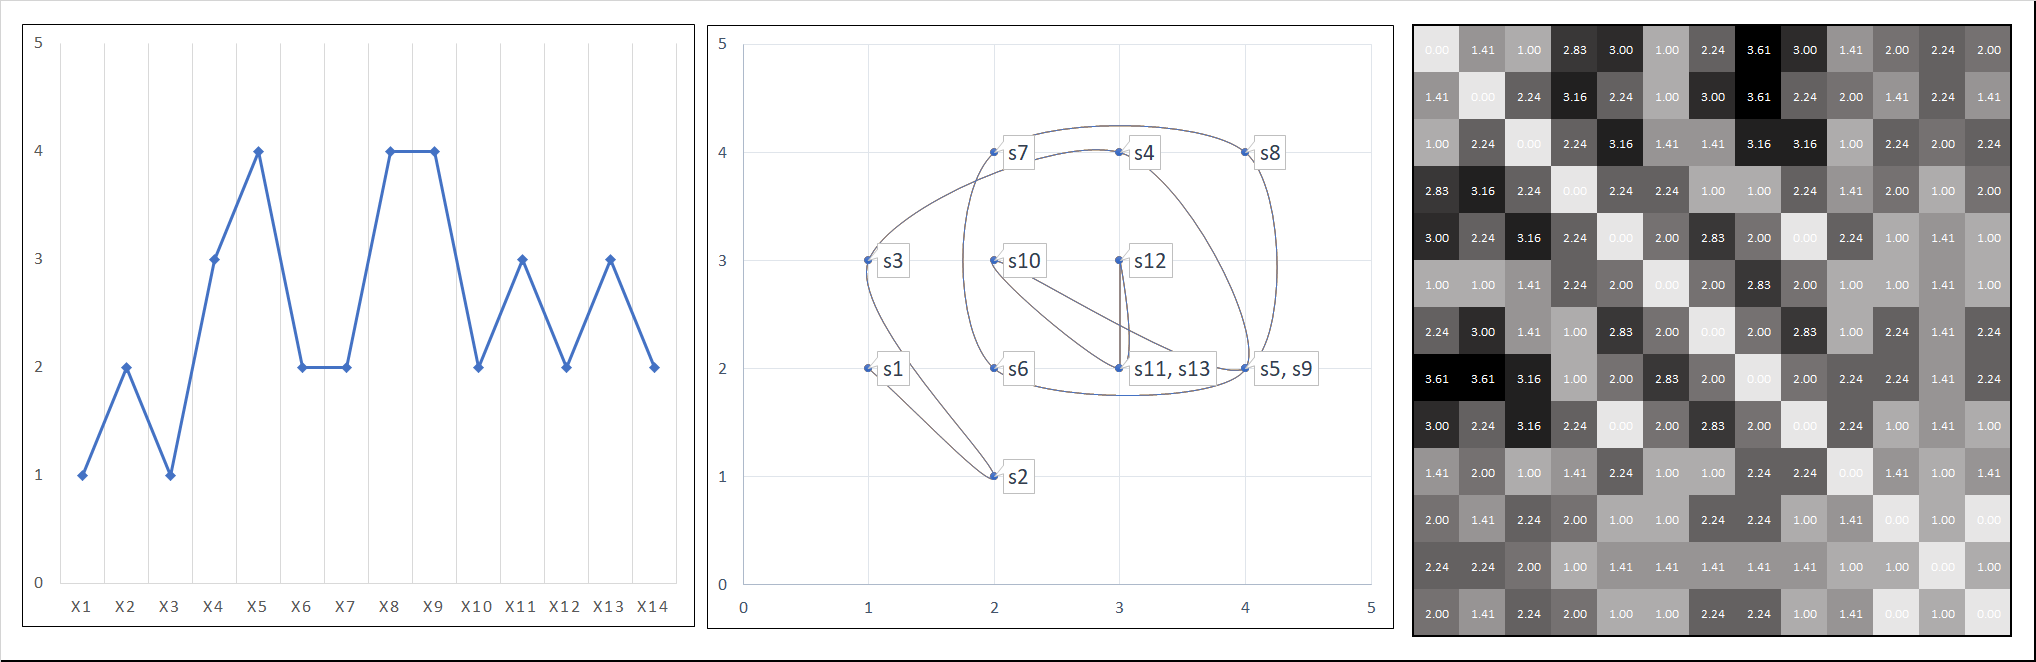
\includegraphics[width=\textwidth]{images/RP.PNG}
    \caption{The left plot shows a time series of seven observations $x_t$, $t=1,\dots,7$. The plot in the middle shows the two dimensional phase space trajectory that is created from $x$ using a time delay of $\tau = 1$. The states are denoted by $s_k$ for $k=1,\dots,6$ where $s_k = (x_k, x_{k+1})$. On the right, the recurrence plot is a matrix of Euclidean distances between the six states: $R_{i,j} = Euclidean(s_i,s_j)$.}
    \label{fig:RP_Def}
\end{figure}

After the recurrence plots are created, we scale them to fall in the interval $[0, 1]$ using the appropriate min-max scaling introduced in Equation \ref{eq:minmax} which is a requirement of the CNN input. 

As it is pointed out in \cite{hatami2018classification}, time series tend to show recurrent behaviour like periodicity, and this phenomenon is generally present in dynamic nonlinear systems or stochastic processes that generate the series. The recurrence plot, as described previously via Figure \ref{fig:RP_Def}, reveals which are the phases that trajectories tend to return to. To attain such a plot, each element of it is the result of this formula:
\begin{equation}
\label{eq:RP_R}
    R_{i,j} = \theta(\epsilon-||\vec{s}_i - \vec{s}_j||),\quad \vec{s}(.) \in \mathbb{R}^m, \quad i,j = 1,\dots,K
\end{equation}
where K is the number of considered states $\vec{s}$, $\epsilon$ is a threshold distance, $||.||$ a norm (Euclidean in our case), and $\theta(.)$ the Heaviside function\footnote{The Heaviside function is defined as: $\theta(x) = \frac{d}{dx}\max(0,x)$ for $x \neq 0$}. Summing up the process of creating a recurrence plot for our purposes: first, we start out with a window containing $30$ consecutive return values of an asset; then we create the two-dimensional phase space trajectory ($m=2$) from these series which results in $29$ states; finally, the R-matrix is calculated based on Equation \ref{eq:RP_R} but with a small change. 
The formula, due to the $\epsilon$ threshold parameter, would give us a matrix of ones and zeros, and to avoid this information loss we simply skip this step and work with the resulting grey-scale images. Also, we use min-max scaling on each resulting image of $(29 \times 29)$ to $[0, 1]$ in order to satisfy the requirements of the CNN's input vectors. 
Afterwards, to fit the image size of the two other transformation strategies introduced later, we add a size $1$ zero-padding to the right and bottom of the image. Zero-padding here is an additional column and row of zeros added to two neighboring sides of the image to increase its size without modifying the resolution or information content of the original image. Visually, it is a column and row of zeros on the right and bottom sides of our RP image.

% potentially mention RP on prices that increase or decrease similar while on returns it is more distinctive

Another image transformation used is the \textbf{Gramian Angular Field (GAF)} that translates the typical Cartesian coordinates into a polar coordinate system. The technique is introduced in \cite{wang2015encoding}, and is based on the Gramian matrix (named after J{\o}rgen Pedersen Gram), the entries of which are given by $G_{ij} = \langle v_i,v_j \rangle$ for a set of vectors $v_1,\dots, v_n$. These entries are inner products which measure the "similarity" of the two vectors. The Gram matrix is generally used for the calculation of the linear independence of a set of vectors. A beneficial property of the Gram matrix is that it preserves temporal dependency in the geometrical setting of the matrix, time flows from the top left to the bottom-right. For example, the Gramian matrix of a univariate time series: $x_t$ for $t=1, 2, 3$ can be computed as:

$$
G =\begin{pmatrix} 
\langle x_1,x_1 \rangle & \langle x_1,x_2 \rangle & \langle x_1,x_3 \rangle \\
\langle x_2,x_1 \rangle & \langle x_2,x_2 \rangle & \langle x_2,x_3 \rangle \\
\langle x_3,x_1 \rangle & \langle x_3,x_2 \rangle & \langle x_3,x_3 \rangle \\
\end{pmatrix}
$$

As noted in \cite{gaf_medium} the use of the Gramian matrix can be motivated by the fact that plain univariate time series prove unsuccessful in explaining co-occurence and latent states in the data and the Gramian matrix provides an alternative visualization. This same article also shows that the traditional Gram matrix is unsuccessful in making a distinction between the Gaussian noise and the valuable information in the data, thus the entries of the GAF matrix are not simply given by the inner product (in an Euclidean setting). Following the definition in \cite{wang2015encoding}, to create a GAF plot from a time series $X = \{x_1,x_2, \dots x_n\}$ of n valued real observations, we first rescale $X$ using min-max scaling to the $[-1,1]$ interval, as described previously in Equation \ref{eq:minmax}, and end-up with the scaled series $\Tilde{X}$. Now, we transform the time series into polar coordinates:
\begin{align}
\label{eq:gafencode}
    \begin{cases}
        \phi_i = \arccos(\Tilde{x}_i), \quad -1 \leq \Tilde{x}_i \leq 1, \quad \Tilde{x}_i \in \Tilde{X}\\
        r_i = \frac{t_i}{N}, \quad t_i \in \mathbb{N}
    \end{cases}
\end{align}
i.e. we convert the timestamp $t_i$ dividing by $N$ (the number of series instances) and get the radius. This means that the radius is longer for values at later time steps. As for the angles, they are the angular cosine of the scaled series. Then, we create the Gramian Angular Field by taking the cosine sum between each pair of angles:

\begin{equation}
\label{eq:GAF}
    GAF =\begin{pmatrix} 
\cos(\phi_1 + \phi_1) & \cdots & \cos(\phi_1 + \phi_n)\\
\cos(\phi_2 + \phi_1) & \cdots & \cos(\phi_2 + \phi_n)\\
\vdots & \ddots & \vdots\\
\cos(\phi_n + \phi_1) & \dots & \cos(\phi_n + \phi_n)\\
\end{pmatrix} \\
= \Tilde{X}' \cdot \Tilde{X} - \sqrt{I-\Tilde{X}^2}' \cdot \sqrt{I-\Tilde{X}^2}
\end{equation}
where $I$ is the row vector $[1, 1, \dots, 1]$. Notice, that this is a Gramian-like matrix with a penalized inner product given by\footnote{Please see Appendices \nameref{app:GAF} for the proof.}: $\langle x, y\rangle - \sqrt{1-x^2} \cdot \sqrt{1-y^2}= x \cdot y - \sqrt{1-x^2} \cdot \sqrt{1-y^2}$. There are several advantages to this construction one of which is preserving the absolute temporal relations. Another aspect is that the diagonal sustains the original (although transformed) time series. Furthermore, the entries $GAF_{ij}$ of the matrix represent the temporal correlation (cosine-similarity) with respect to the different $k= |i-j|$ time intervals, and the main diagonal displays the case of $k=0$. Figure \ref{fig:GAF} shows how the transformation happens for an example scaled time series of $14$ observations. Time can again be tracked going from the top-left to the bottom-right corner.

\begin{figure}[!htb]
    \centering
    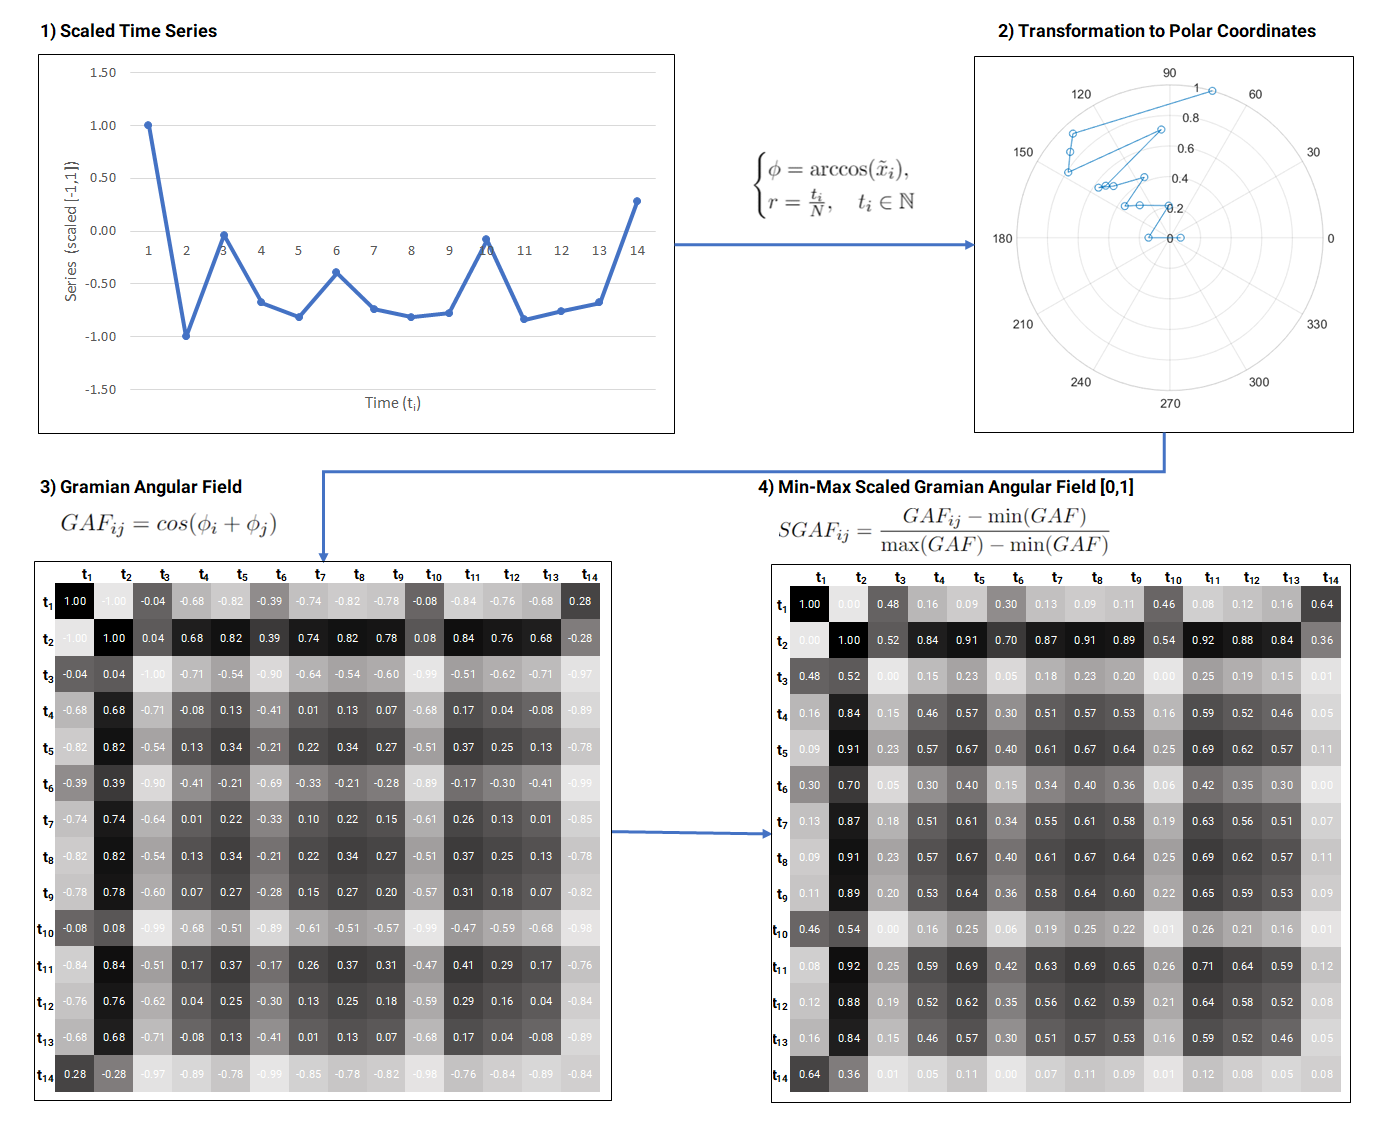
\includegraphics[width=\textwidth]{images/GAF.png}
    \caption{Plot 1 shows the time series scaled to the interval [-1, 1] which is then transformed to polar coordinates. In the polar coordinate system in Plot 2, the first point is the closest to the center, then as time moves forward, the coordinates vary among different angles but move further and further out towards the boundaries of the unit circle. Plot 3 shows the GAF plot that we get by applying the formula in Equation \ref{eq:GAF}. Before applying the CNN, we use min-max scaling to the interval $[0,1]$ to fit the expected input of the model. As Plot 4 demonstrates, this scaling does not change the appearance of the image.}
    \label{fig:GAF}
\end{figure}

The third and last transformation strategy introduced is called \textbf{Markov Transition Field (MTF)} and it entails encoding dynamic transition probabilities from a Markov Transition Matrix of discretized quantile bins in a quasi-Gramian matrix. The algorithm is introduced in \cite{wang2015encoding} and inspired by \cite{campanharo2011duality}.

In its essence, the method consists of encoding the dynamic transition probabilities in a Markov Transition Matrix and then from that matrix create a new one that also preserves information about the sequentiality of the time series which is the MTF.
To be more precise, given a time series $X_t$ (which, in our case, is the return series) we first identify its $Q$ quantile bins $q_j$ $(j \in [1,Q])$. In Figure \ref{fig:MTF}, Plot 1 illustrates this step. Afterwards, matrix $V$ is a $Q \times Q$ weighted adjacency matrix, with $V_{ij}$ representing the count of transitions from $q_i$ to $q_j$ within one time step. 
%This is also a first-order Markov chain along the time axis.
Then, the Markov Transition Matrix denoted by $W$ is constructed by normalization of $V$:

\begin{equation}
\label{eq:W}
    W_{ij} = V_{ij}/\sum_j V_{ij}.
\end{equation}

Thus, $W_{ij}$ gives us the probability of moving from the $i^{th}$ bin to the $j^{th}$ bin within one time step. Now, the issue with this matrix is that we lose a lot of information and it fails to represent that the data is serial in time. Therefore, \cite{wang2015encoding} suggests a design that sustains the time dependence via the locations of the values in the matrix. The Markov Transition Field can then be described as:

\begin{equation}
    \label{eq:MTF}
        MTF =\begin{pmatrix} 
    W_{ij|x_1 \in q_i, x_1 \in q_j} & \cdots & W_{ij|x_1 \in q_i, x_n \in q_j}\\
    W_{ij|x_2 \in q_i, x_1 \in q_j} & \cdots & W_{ij|x_2 \in q_i, x_n \in q_j}\\
    \vdots & \ddots & \vdots\\
    W_{ij|x_n \in q_i, x_1 \in q_j} & \dots & W_{ij|x_n \in q_i, x_n \in q_j}
    \end{pmatrix}
\end{equation}
and an example can be observed in Plot 3 of Figure \ref{fig:MTF}. This resulting image, similarly to the previous two representations trails the flow of time from the top-left to the bottom-right corner.
The entries of this matrix are already in the range $[0,1]$, so there is no need for further scaling before feeding it to the CNN. The images are created with the same sliding window technique discussed previously. A parameter to decide on is the number of quantile bins to create, and with window size set to $30$ it is set to five in our image construction.\footnote{It should be noted that the number of bins can be optimized via costly hyperparameter optimization but due to limitations in time and computational power this was not carried out in the study.}
The MTF can also be understood as the multispan transition probabilities of the series within one step at different points in time.

\begin{figure}[!htb]
    \centering
    
\includegraphics[width=\textwidth]{images/MTF.png}
    \caption{Plot 1 shows the time series which is assigned to $Q=4$ quantile bins. In Plot 2.a), we can inspect the preliminary state of the Markov Transition Matrix $V$, the elements of which are the counts of the different transitions in the time series $X$, and in Plot 2.b) $W$ is the so-called right stochastic matrix or Markov Transition Matrix, a real stochastic matrix with transition probabilities between the different bins and each row summing to $1$ (see Equation \ref{eq:W}). Plot 3 shows the MTF plot that we get by applying the formula in Equation \ref{eq:MTF}.}
    \label{fig:MTF}
\end{figure}

Overall, the three representations have some common properties, such as how the time dimension is represented in the way the different pixels are located. Also, all three methods provide us a way to transform sliding windows of time series into graphical representations that an image classifier can potentially recognize given proper labels. However, all three transformations show us a slightly different aspect of the series. While the recurrence plot highlights cyclicality and recurring patterns in the data, the GAF illustrates temporal dependencies and the MTF reveals the transition-related behavior in the series. Figure \ref{fig:allTrf} shows an example of all three transformations on the same return series of length $30$.

\begin{figure}[ht]
    \centering
    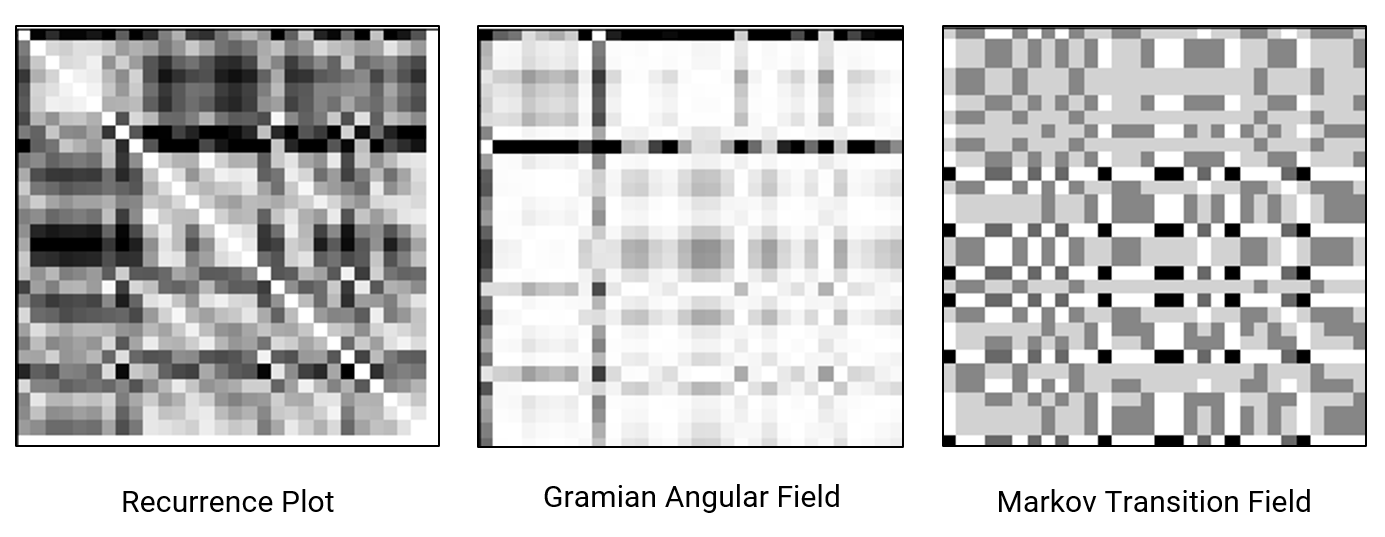
\includegraphics[width=\textwidth]{images/allTrf.PNG}
    \caption{Recurrence Plot, Gramian Angular Field and Markov Transition Field applied on the same return series consisting of 30 observations.}
    \label{fig:allTrf}
\end{figure}

\subsection{Image Labelling}
\label{subsec:DM:IL}
The image labelling is done in two steps. First, we label the original time series and, in a second step, the images using the labels from Step 1.
The labelling algorithm is based on a simple idea and follows the one applied in \textit{Algorithm 1 in} \cite{sezer2018algorithmic}.

The algorithm for the time series is as follows. We choose an odd labelling window size $l = 5$. The oddness is required since we slide this labelling window along the series and label the middle element of the window as "Buy" ("Sell") if the mid point of the window is the minimum (maximum) of the values in the window, otherwise they are "Hold". The process is illustrated in Plots 1-6 in Figure \ref{fig:Labelling}. 
Two special cases are when, after a plunge, the series remains constant and then goes up again, and vice versa. They are also shown in Plots 7-10 in Figure \ref{fig:Labelling}, and the rule is as follows: 
given the middle observation in the labelling window is sharing its property of being a local minimum (maximum) with at least one of its direct neighbours, then the label is a "Buy" ("Sell") only if the observation following the mid point is strictly greater (strictly less) than the mid point.

In step two, we digress from the mentioned literature. Each image is labelled as the last element of the series that is used for creating the image. In other words, considering image window size of $s$ and return series $X_t$ for $t = 1, \dots, n$ for $n > s$ which has labels defined by\footnote{The notation $\lfloor \cdot \rfloor$ refers to the floor function.} 
$L_{\bar{t}}$ for 
$\bar{t} = \left(1+\lfloor \frac{l}{2} \rfloor\right), \dots, \left(n-\lfloor \frac{l}{2} \rfloor\right)$ with labelling window size $l$, and each image made up of the subset of the series given by
$X_{(i,\dots,(i+s-1))}$  
for every
$i = \left(1+\lfloor \frac{l}{2} \rfloor\right), \dots, \left(n-s+1-\lfloor \frac{l}{2} \rfloor\right)$ gets the label $L_{i+s-1}$. All in all, this indicates that given a series of $n$ returns, we can label $\left((n - s + 1)-\lfloor \frac{l}{2} \rfloor\right)$ of the $(n - s + 1)$ images created.
There are multiple reasons to pursue this approach. Firstly, if we were to label an image based on the price at its mid point, the prediction of a label would come too late to actually trade at that price. Secondly, the choice of the labelling window size does not have to match the window size used for image creation which is also beneficial because the labelling window size allows us, to some extent, to choose the frequency of "Buy" and "Sell" orders because a smaller window size identifies more of them. 

\begin{figure}[ht]
    \centering
    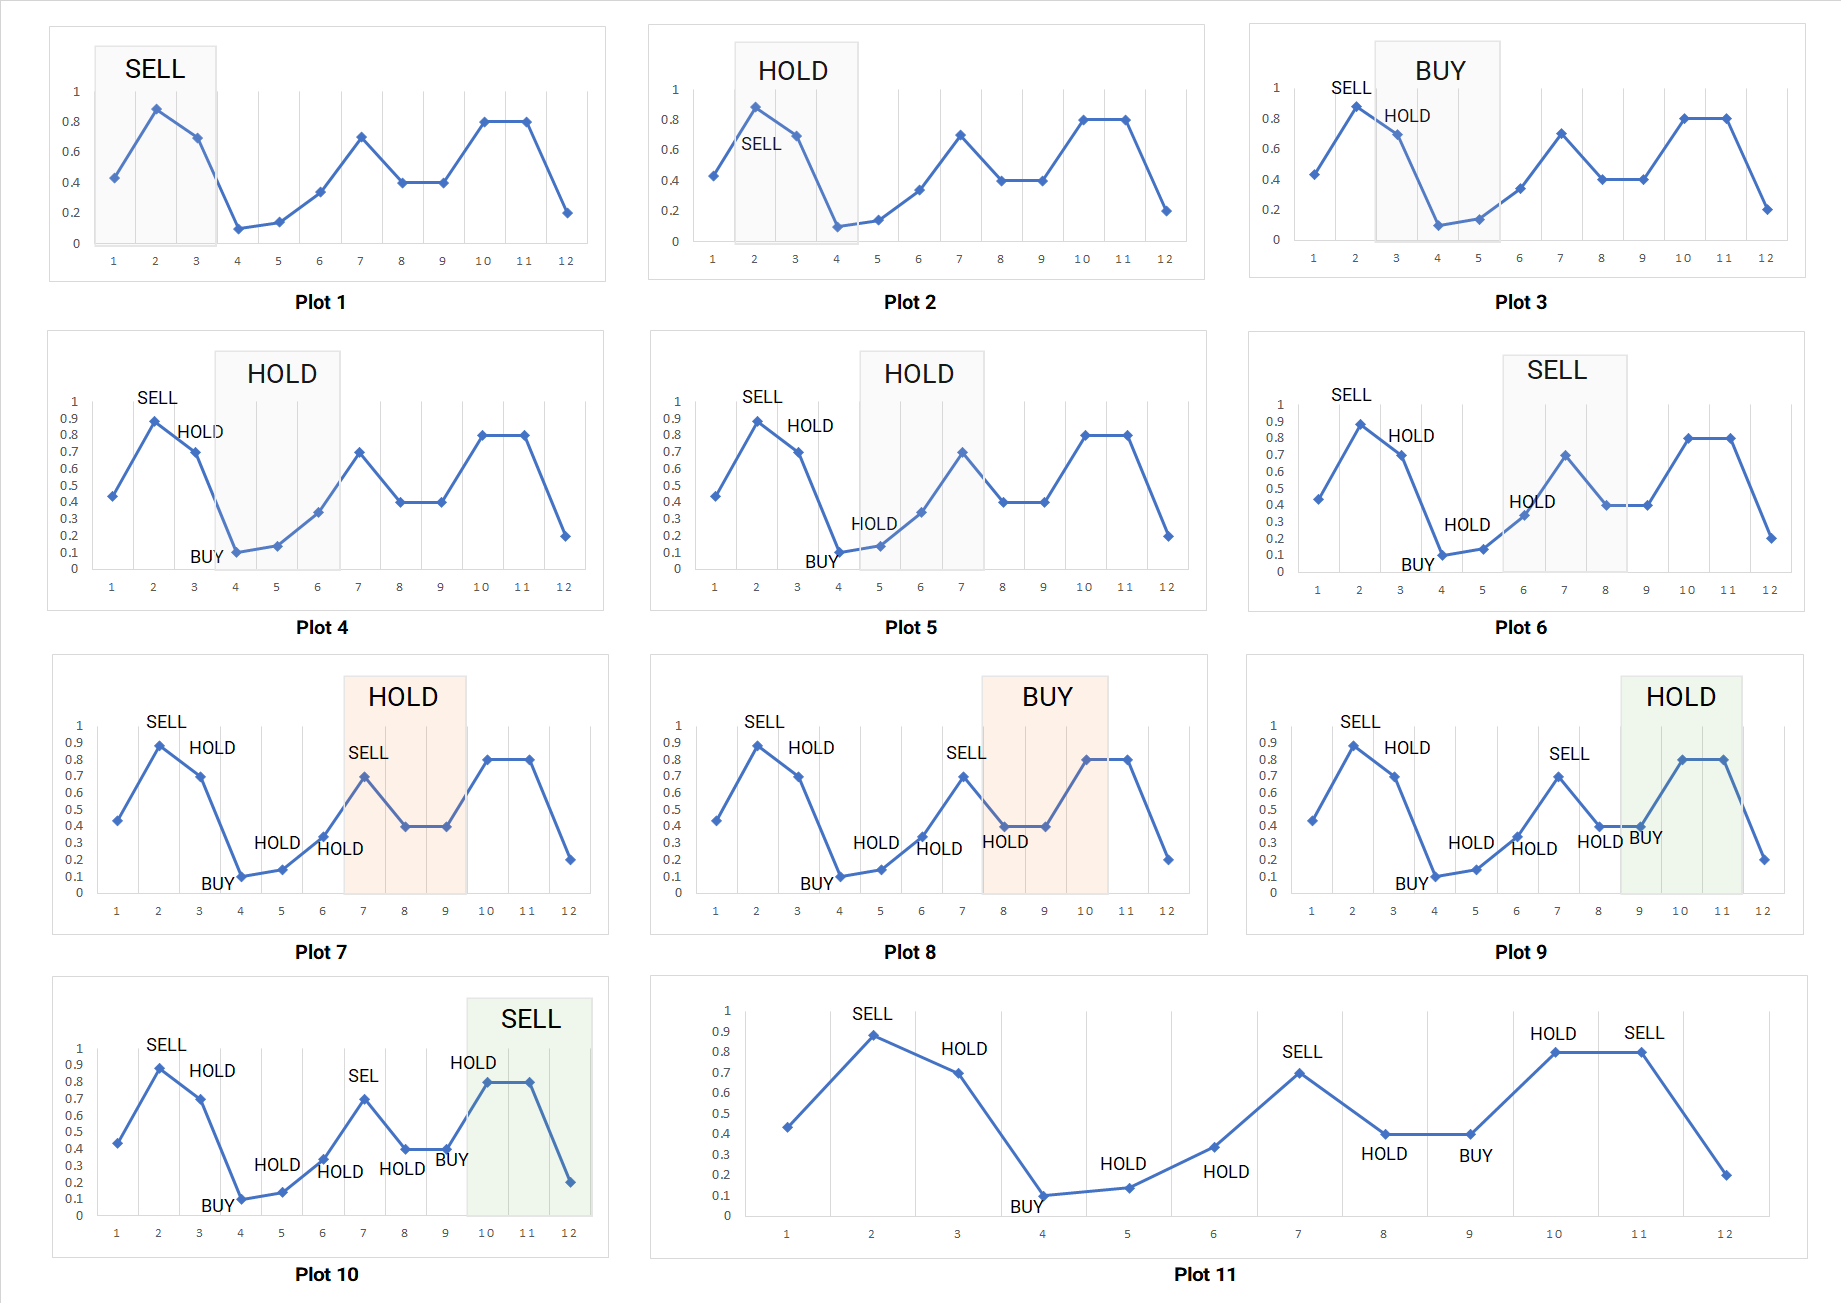
\includegraphics[width=\textwidth]{images/Labelling.png}
    \caption{Example of labelling. The figure visualizes the step-by-step labelling of an example series of $12$ observations with labelling window of size $l=5$. The grey rectangles show the scope of values considered in every labelling decision, and that the value in the middle time step is labelled in every step (Plots 1-6). Plots 7-8 show the process in the first special case, that is when the mid value is not the only local minimum, but shares this property with one of its neighbouring observations. The decision in the second special case, depicted in Plots 9-10, is similar, only with two consequent local maxima within the same window. It can also be seen in Plot 11 that the first and last $\lfloor \frac{l}{2} \rfloor = 1$ values cannot be labelled.}
    \label{fig:Labelling}
\end{figure}

\subsection{Recognizing Patterns with Deep CNN}
\label{subsec:DM:RecPatwCNN}

Deep convolutional neural networks are artificial neural networks (ANN) with multiple layers between the input and output layers (hence deep) that also employ convolution operation in one or more layers as a substitute for the matrix multiplication (see p.326, Chapter 9 in \cite{goodfellow2016deep}). 
The CNN has many advantageous properties but what is most important for our use-case is that it can process fairly raw high dimensional data and extract the most important features for the given exercise. It accomplishes this by the use of filters which change the original input in different ways in an attempt to learn relevant features for solving the problem. 
An example of a $2 \times 2$ filter could be a blurring filter, that moves along all the $2 \times 2$ neighboring pixels of an image. When it finds a distinctive contrast in color between the four ($2 \times 2$) neighboring pixels, it changes their color so they fall a bit closer to each other. Moreover, the sparse connectivity in the network prove to be computationally more efficient and better in generalization when compared with multilayer perceptrons (MLP).\footnote{On how generalization is improved by removing redundancies see \cite{chakraborty1999effect}.} 
As it is also described in \cite{MLPmedium}, MLPs are fully connected neural networks with at least three layers (input, hidden and output) and the issue with fully connectedness is that the number of parameters equals the product of parameters on the different layers and this can increase very quickly with more complicated networks. 
It is inefficient due to redundancies in the network, also, MLPs flatten the output of each layer before feeding into the next one which disregards spatial information. The CNN however can account for local connectivity (see orange and green filters in Figure \ref{fig:CNNstruct}), the weights are shared (strolling the same filters over the entire image), and as for being sparse, each neuron in a layer is not connected to each neuron in the neighbouring layer. 
Deep neural networks have many constituents that shall be chosen for the data and objective of the model. Below we will get an overview of these choices and the final model design (also see Figure \ref{fig:CNNstruct}).

The first component that we discuss is the activation function which has an important role in introducing non-linear properties to the neural network. The activation function that is used throughout the models is Leaky ReLU, which is a version of the commonly used ReLU function. ReLU stands for rectified linear unit (\cite{hahnloser2000digital}) and is defined as
\begin{equation}
    \label{eq:ReLU}
    y = f(x) = \max(0,x).
\end{equation}
The ReLU is popular as it prevents against vanishing gradients (\cite{glorot2011deep}) and it has a low computational cost. Lastly, it promotes sparsity since all negative inputs result in zero activation which helps the model in finding meaningful features faster and prevents against overfitting. 
On the other hand, the fact that all negative results are turned into zero can be an issue when a value keeps giving negative results. In this case the ReLU turns it into zero every time and due to not being any slope below zero the neuron is very likely to remain inactive for the rest of the training. 
This way, these neurons will have no contribution to the network and this is an even bigger problem if more and more neurons turn up "dead". To prevent against the described disadvantages we use Leaky ReLU which solves the issue by introducing a slope in the negative side of the function (\cite{maas2013rectifier}):
\begin{equation}
    \label{eq:LeakyReLU}
    y = f(x) = 
   \begin{cases*}
      x & \text{if $x \geq 0$} \\
      \alpha x        & \text{if $x<0$}
    \end{cases*}
\end{equation}
where we use $\alpha = 0.3$. The Leaky ReLU also helps accelerating the training process as it is more balanced than the simple ReLU. On the output layer we apply softmax activation that is usually used for multiclass classification problems as it normalizes the outputs of the last layer so it becomes a probability distribution over $K$ classes. The standard softmax function is $\sigma: \mathbb{R}^K \rightarrow \mathbb{R}^K$
\begin{equation}
    \label{eq:softmax}
    \sigma(\mathbf{z})_i = \frac{e^{z_i}}{\sum_{j=1}^K e^{z_j}} 
\end{equation}
for $i = 1,\dots, K$ and $\mathbf{z} = (z_1, \dots, z_K) \in \mathbb{R}^K$.\footnote{For more on the softmax activation function please see \cite{nielsen2015neural}}

For regularization, three different methods were implemented: batch normalization, dropout layers and L2 kernel regularization. The batch normalization (\cite{ioffe2015batch}) is both useful to regularize the network and it improves training speed and performance by normalizing the input for each layer in the network for each mini-batch. This is used to avoid the problem of the varying distribution of input during training. The dropout (\cite{srivastava2014dropout}) is a method to reduce overfitting by randomly dropping nodes together with their connections from the network during training with a given drop-probability. The technique works by preventing co-adaptation among units (for more on the topic please see \cite{hinton2012improving}). The third regularization implemented is L2-regularization (or Ridge Regression) which works by penalizing the loss function (\cite{ng2004feature}). This is done by adding the penalty $\frac{1}{2}\lambda w^2$ to the loss function for each weight $w$ with regularization strength $\lambda = 0.01$ in our network. The penalty term helps reducing the role of peaky weights and thus the network pays attention to the nodes in a more balanced fashion.

The loss function is the Kullback-Leibler divergence which, for $n$ prediction vectors $\mathbf{y}^{pred}_i$ ($i= 1, \dots, n$) and $n$ corresponding true value vectors $\mathbf{y}^{true}_i$ ($i= 1, \dots, n$), is given as
\begin{equation}
    \label{eq:KL}
    Loss_{KL} = \sum_{i=1}^{n}\mathbf{y}_i^{true} \log \left( \frac{\mathbf{y}_i^{true}}{\mathbf{y}_i^{pred}}\right)
\end{equation}
and it measures the similarity between the true and predicted distributions. This loss function was selected based on empirical findings, on multiple trials, the model training showed a better convergence with less fluctuation using this function versus the categorical crossentropy.

As optimizer we apply Stochastic gradient descent (SGD) and for the optimization of this algorithm, Nesterov accelerated gradient (NAG). This was chosen by model tuning, generally this setting provided a faster convergence than Adam, Nadam or RMSProp. The SGD update for $w$ parameter at the $k^{th}$ iteration is
\begin{equation}
    \label{eq:SGD}
    w_k = w_{k-1} - \eta_{k-1} \cdot \nabla f(w_{k-1})
\end{equation}
where $\eta$ is the learning rate and $\nabla f(w_{k-1})$ is the stochastic gradient at $w_{k-1}$. With the NAG we break this update into two parts. The Momentum optimization (first introduced by \cite{polyak1964some}) of SGD accelerates the optimization but it also makes it prone to overshooting. The NAG is similar to the Momentum, it also breaks the parameter update into two equations:
\begin{align}
\label{eq:NAG}
    \begin{split}
        v_t &  = \gamma v_{t-1} - \eta_{t-1} \nabla f(w_{t-1} + \gamma v_{t-1}) \\
        w_t & = w_{t-1} + v_t 
    \end{split}
\end{align}
where $\gamma$ is the momentum term determining how much of the previous time step's update vector is represented in the current update vector. In the Momentum method this induces the acceleration to the right direction. Since we use $\gamma v_{t-1}$ to change the $w_t$ parameters, the expression $w_{t-1} + \gamma v_{t-1}$ is an approximation of the next position of the parameter and this is used for calculating the gradient instead of the current parameters (\cite{ruder2016overview}).

\begin{figure}[ht]
    \centering
    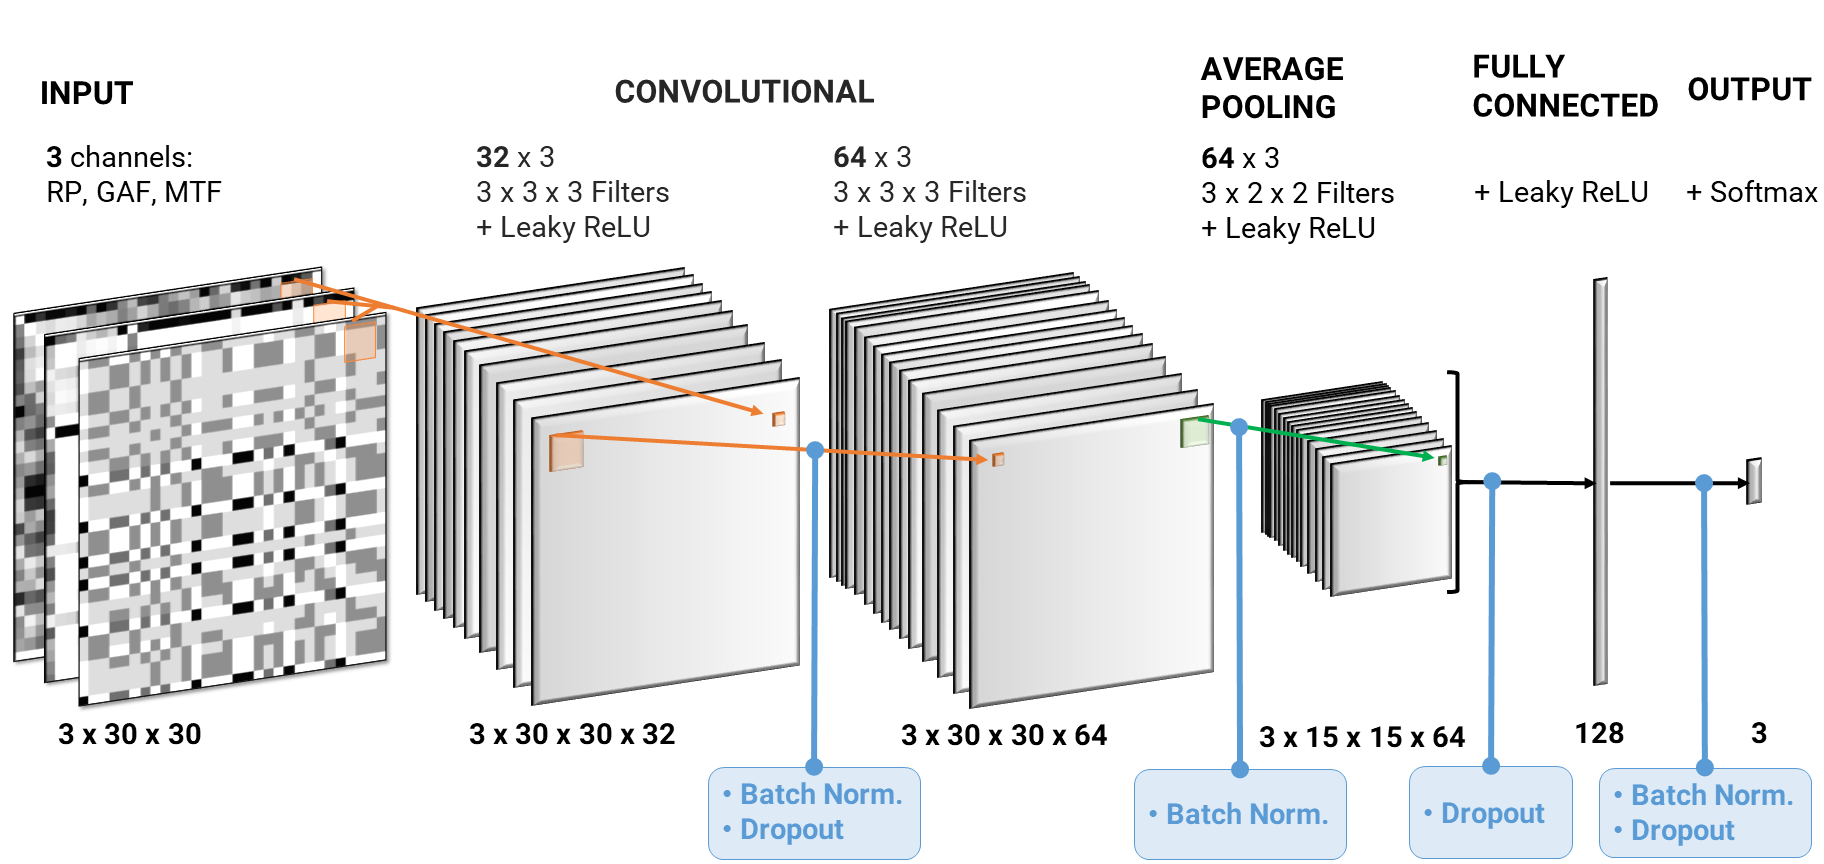
\includegraphics[width=\textwidth]{images/CNNCtrf.png}
    \caption{The basic structure of the Convolutional Neural Network used for trading order prediction}
    \label{fig:CNNstruct}
\end{figure}

To further facilitate the understanding of the model, the general visualization of deep neural networks is used to depict its architecture in Figure \ref{fig:CNNstruct}. For each window of 30 subsequent return values the 3 image representations (each of size $30 \times 30$) are fed to the model through the color channels serving as an input. These are then filtered with $32$ kernels of size $3 \times 3 \times 3$ (using zero padding to maintain image size, and the stride is 1) which gives us 32 convolutional layers of size $3 \times 30 \times 30$. It is worth to note that we use small filters due to our images being also relatively small. 
The activation map of the layers is obtained by using Leaky ReLU, described previously in Equation \ref{eq:LeakyReLU}, preceded by batch normalization in order to prevent against overfitting. This is further supported by a dropout layer with $0.3$ drop rate \footnote{The drop rate in the first and second dropout layer is $0.3$ for each model built on individual assets but it varies according to tuning in the universal model builds ($0.25$ in certain periods).}. 
Next, we have 64 convolutional layers of size $3 \times 30 \times 30 \times$ created using filters with the same characteristics as before (including stride and zero padding). This is followed by batch normalization, and then the activation map is once again made using the Leaky ReLU function. After, these convolutional layers are average pooled with $3 \times 2 \times 2$ kernels which results in 64 layers of size $3 \times 15 \times 15$ on which we again apply the Leaky ReLU followed by a second dropout. 
The information from these layers is condensed by the flattening of the the feature map (output resulting from previous layer) and feeding it to the fully connected layer of size $128$. This is also followed by batch normalization and dropout with $0.5$ drop rate for asset-specific models and $0.3$ or $0.25$ drop rates for the universal models. The decreased dropout is sufficient for the universal asset model due to the larger amount of training data already aiding generalization capabilities. Finally, there is the output layer with softmax activation that gives us the probabilities for each image being "Sell", "Buy" or "Hold" class. 
The described architecture reflects the basic build of each model that has been trained and tested. Some hyperparameters and further settings were customized in the tuning phase for each model. 
Such aspects include the class weights applied in the loss function (as there is an imbalance between the three classes), mini-batch sizes, hyper-parameters of the objective function, dropout rates and L2 regularization strength. The weighted loss function is similar to that in \ref{eq:KL} but each element of the sum is weighted with the predefined weight of the true class. Thus more weight is added to the smaller "Buy" and "Sell" classes ensuring that they are sufficiently represented in the losses.

We attempted to train deeper models (with more hidden layers) and wider models (with more neurons per layer) but the networks did not improve the results of this smaller network, moreover, in some cases they even showed reduced generalization capability. This is commonly reported in deep learning research (\cite{ObrienStack}), and the explanation is that, up to a point, increasing the complexity of a network help learning more abstract features and more combinations of these features, but it also encourages memorization instead of learning broader rules thereby limiting generalization. Thus, we adopted a simpler high level model skeleton that is common in the field, similar to that in \cite{sezer2018algorithmic}, but with a customized mix of components as specified above.

\subsection{Evaluation Techniques}
\label{subsec:DM:Eval}

For assessing the technical performance of the CNN, we use accuracy, class-wise and average precision, recall and F1 scores, moreover we will also present the confusion matrix for the different models and testing periods. 
The confusion matrix allows us to observe the absolute number of correctly and wrongly classified observations by classes. 
\begin{figure}[ht]
    \centering
    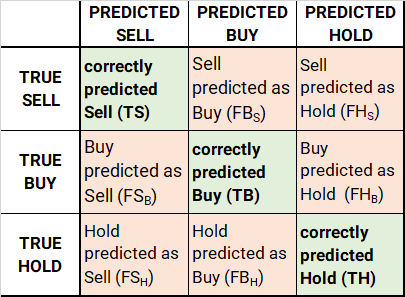
\includegraphics[width=.5\textwidth]{images/Confusion_matrix.png}
    \caption{The structure of the confusion matrix. The notations "TS", "TB", and "TH" mean True Sell, True Buy and True Hold, while "FS", "FB", and "FH" mean False Sell, Buy, and Hold, the subscript refers to the true class in case of false classification.}
    \label{fig:cmdef}
\end{figure}
The matrix that we will see in the section \nameref{subsec:ER:ClassPerf} has the structure described in Figure \ref{fig:cmdef}.
The accuracy tells us about the proportion of observations that is classified correctly over all the classes $k = \{S, B, H\}$ . Now, given we wish to calculate measurements for a classification on a set of $N$ values, i.e. $N = TS + TB + TH + \sum_k \left(FS_k + FB_k + FH_k\right)$ using the notations in Figure \ref{fig:cmdef}, the accuracy is:
\begin{equation}
    \label{eq:acc}
    Accuracy = \frac{TS + TB + TH}{N}
\end{equation}
the class-wise precision for each class $K$ is given by
\begin{equation}
    \label{eq:pr}
    Precision_K = \frac{TK}{TK +  \sum_k FK_k}
\end{equation}
and the class-wise recall is then 
\begin{equation}
    \label{eq:rec}
    Recall_K = \frac{TK}{TK +  \sum_{k  \smallsetminus \{K\}} Fk_K}
\end{equation}
or in other words, the precision of a class $K$ tells us the proportion of correct classifications among all the predictions of $K$, and the recall gives the percentage of the true $K$ class that is correctly classified as $K$. The F1 score is a useful measurement in unbalanced classification tasks, and it is the harmonic mean of the precision and the recall in every class:
\begin{equation}
    \label{eq:f1}
    F1_K = 2 \frac{Precision_K \cdot Recall_K}{Precision_K + Recall_K}.
\end{equation}
We will also see macro average results over the classes for each of these metrics which means the average of the classwise metric results, e.g. the macro average for the F1-score is $\frac{F1_S + F1_B + F1_H}{3}$.

Furthermore, financial assessment is carried out on the test data which we start by setting an initial capital of $C_0 = 10000$ and a flat transaction based trading commission of $c = 5$ (both in USD). At every time step $t$ the trading orders are executed as per the signals ($s_t$) at price $p_t$ which are predicted by the model for the respective time step.
In case of repeating consequent signals, the first signal prompts a trading action given cash/the asset is available in holdings. The Buy order is completed given money is available (up until the first Buy order, and after each executed Sell) and the Sell order is completed if units of the financial instrument are available for selling (i.e. after each executed Buy), otherwise they are handled as a Hold. In case of a Hold signal at $t$, trade does not take place, only the amount of capital $C_t$ is tracked at the given period. As a safety feature, to avoid obvious mistakes by the model, a "Buy" order is only executed if the current price is not higher than the previous and a "Sell" order is only executed if the current price is not lower than the previous.
Assets are assumed to be traded in any increments. Using the described approach over the period $t=1, \dots, T$ the following measurements are calculated for the financial performance evaluation:

\begin{itemize}
    \item number of all executed trades: $n_{trade}$
    \item total profit/loss: 
    \begin{align}
        \label{eq:totPL}
            P\& L = C_T - C_0
    \end{align}
    \item cumulative return: 
    \begin{align}
        \label{eq:cumret}
            r_c = \frac{P \& L}{C_0}
    \end{align}
    \item annualized return (for business year of 260 days): 
    \begin{align}
        \label{eq:annualized}
            r_{ann} = \frac{C_T}{C_0}^{\frac{260}{n}}-1
    \end{align}
    \item average P \& L per trade:
    \begin{align}
        \label{eq:avgpl}
        AvgP \& L = \frac{P \& L}{n_{trade}}
    \end{align}
\end{itemize}

To monitor the performance over different economic regimes, we test the model throughout approximately 2 year periods in 2006-2007, 2008-2009 and May 2017 - June 2019. The first testing period is one before the crisis, the second one is during the financial crisis and the latest is to show current market conditions. 
The models will be trained on all previous available data up to the first day of testing. 
Moreover, the evaluation of competing algorithmic trading techniques, for the same testing periods with the same financial metrics provided in Equations \ref{eq:totPL} - \ref{eq:avgpl}, are carried out to make the evaluation more comprehensive.
There are three methods considered for comparison: the Buy \& Hold, the momentum-based Relative Strength Index (RSI), and a volatility-based strategy using the Bollinger Bands (BB).\footnote{The strategies are described in the Appendices: \nameref{app:CompetingStrats}}

In order to assess feasibility we will also present how much time it takes for the model to train and to return predictions from the trained model. Since creating new image representations is part of making a new trading decision every time a new value appears in the time series (e.g. new daily price), we will also check how long this image creation phase takes.
The execution time for image creation will be shown in milliseconds per generation of a new image instance, with turning the price series into a return series and then creating all three variations of the image: RP, GAF and MTF. The values are calculated for different image sizes and they are the mean execution times from 1000 runs for each image size.

It is important to note that all presented results in the paper are biased to some extent, because if one would wish to create unbiased results, each model would need to be run many times with different validation sets. This way, using all results we could assess the overall average performance and via standard deviations we could see how stable/robust the results are. However, making these unbiased results requires excessive computational resources and time which is not given within the scope of this research. Such detailed assessments can be a part of future researches. In this paper, the mentioned issue is partially overcome by testing on different asset classes and time periods.

In addition, both in case of the classification results and the financial results we will carry out a dependent, two-tailed Student's t-test for paired samples (\cite{student1908probable}) in order to find out if the results are significantly different from each other for the different models. In case of the classification, the t-test will show us for each period if the mean accuracy, F1-score, precision and recall are significantly different from each other for the universal versus the asset-specific model build. For the financial results, a similar test will be carried out to see if the different model variants produce significantly different mean annual returns in each testing period. The metrics that we will run the tests on are all numeric and continuous, thus the difference of each pair of these metrics is continuous as well. We also assume that the differences of the measurements in each pair of observations are coming from a normal distribution, and that each pair is independent from another. The null-hypothesis for each comparison will be that the mean of the measurements for the given metric is the same for the compared model variants. The alternative hypothesis is that they differ. In the \nameref{sec:ER} section, the p-values will be displayed. All of these p-values will give the probability of observing the test results under the null-hypothesis. The test statistic is calculated for a metric $M$ for model variants $a$ and $b$ and for measurements $i = 1, \dots, n$ the following way. First, we calculate the differences: for each $i$, $M_i^D = M_i^a - M_i^b$, then we calculate the mean ($\bar{M}^D$) and the standard deviation ($s^D$) of the observations $M^D_i$, $i = 1, \dots, n$, and we use them to return the test statistic:
\begin{equation}
    \label{eq:ttest}
    t = \frac{\bar{M}^D}{s^D / \sqrt{n}}
\end{equation}

which then can be used to get the two-tailed p-value, $p = 2* Pr(T > |t|)$, where $T$ is the critical value of the Student t distribution with $n-1$ degrees of freedom. We note, that the sample size of altogether five-five observations per test is very small but, with the above assumptions, the results should be good enough for supporting the comparison process.

\section{Results}
\label{sec:ER}

In this section we cover the main results of the asset-specific and universal model, together with the financial results of the competing strategies. In the following section, we will discuss the reasons behind the results and their implications.

\subsection{Classification Performance}
\label{subsec:ER:ClassPerf}

The classification performance results can be seen in Table \ref{tbl:ClassRes} and Figures \ref{fig:CMAggrI} - \ref{fig:CMAggrU}.
Regarding accuracy, the asset-specific model ended up producing higher test accuracy scores. 

On the other hand, F1, Precision and Recall scores are higher for the universal model setting for almost all periods and assets. In the second testing period, the classification results of the universal model build are generally worse than in either period 1 or 3.

\begin{table}[H]
\begin{tabular}{l|l|cc|cc|cc|cc}
\multicolumn{1}{m{1cm}|}{\multirow{2}{1cm}{Test period}} & \multicolumn{1}{m{1.5cm}|}{\multirow{2}{1.5cm}{Tested Assets}} & \multicolumn{2}{c|}{Accuracy} & \multicolumn{2}{c|}{Average* F1} & \multicolumn{2}{c|}{Average* Precision} & \multicolumn{2}{c}{Average* Recall}  \\
\cline{3-10}
&& CNN-I & CNN-U & CNN-I & CNN-U & CNN-I & CNN-U & CNN-I & CNN-U \\ \hline \hline
\multirow{6}{1cm}{2006-2007} & S\&P500          & 0.51          & 0.45 & 0.36 & 0.45          & 0.36 & 0.43          & 0.35 & 0.46          \\
& Nikkei225        & 0.56          & 0.49 & 0.38 & 0.51          & 0.39 & 0.47          & 0.38 & 0.54          \\
& Nasdaq           & 0.55          & 0.43 & 0.35 & 0.43          & 0.35 & 0.42          & 0.35 & 0.45          \\
& AAPL             & 0.59          & 0.43 & 0.36 & 0.41          & 0.37 & 0.40          & 0.36 & 0.41          \\
& SPY              & 0.57          & 0.44 & 0.38 & 0.47          & 0.38 & 0.44          & 0.38 & 0.50          \\ \cline{2-10}
& \textit{Average} & \textbf{0.55} & 0.45 & 0.37 & \textbf{0.45} & 0.37 & \textbf{0.43} & 0.36 & \textbf{0.47} \\ \hline
\multirow{6}{1cm}{2008-2009} & S\&P500          & 0.52          & 0.35 & 0.37 & 0.38          & 0.37 & 0.38          & 0.38 & 0.38          \\
          & Nikkei225        & 0.53          & 0.35 & 0.35 & 0.39          & 0.36 & 0.39          & 0.35 & 0.39          \\
          & Nasdaq           & 0.59          & 0.38 & 0.35 & 0.41          & 0.35 & 0.42          & 0.35 & 0.41          \\
          & AAPL             & 0.60          & 0.37 & 0.34 & 0.41          & 0.34 & 0.41          & 0.34 & 0.41          \\
          & SPY              & 0.56          & 0.36 & 0.37 & 0.41          & 0.36 & 0.41          & 0.37 & 0.42          \\ \cline{2-10} 
          & \textit{Average} & \textbf{0.56} & 0.36 & 0.36 & \textbf{0.40} & 0.36 & \textbf{0.40} & 0.36 & \textbf{0.40} \\ \hline
\multirow{6}{1cm}{2017-2019} & S\&P500          & 0.59          & 0.44 & 0.38 & 0.52          & 0.39 & 0.48          & 0.38 & 0.57          \\
& Nikkei225        & 0.58          & 0.38 & 0.40 & 0.45          & 0.40 & 0.43          & 0.41 & 0.46          \\
& Nasdaq           & 0.50          & 0.41 & 0.36 & 0.47          & 0.36 & 0.44          & 0.37 & 0.50          \\
& AAPL             & 0.55          & 0.37 & 0.35 & 0.46          & 0.35 & 0.43          & 0.35 & 0.49          \\
& SPY              & 0.56          & 0.42 & 0.37 & 0.49          & 0.36 & 0.45          & 0.37 & 0.53          \\ \cline{2-10}
& \textit{Average} & \textbf{0.56} & 0.40 & 0.37 & \textbf{0.48} & 0.37 & \textbf{0.45} & 0.37 & \textbf{0.51}
\end{tabular}
\caption{Classification results for asset-specific models (CNN-I) and universal models (CNN-U). *Macro average as explained previously.}
\label{tbl:ClassRes}
\end{table}

In Figure \ref{fig:CMAggrI}, we can see the confusion matrix for the asset-specific model aggregated over all periods and testing assets. The matrix shows that most observations are classified as "Hold" which is partially due to the imbalanced data used for training (around 70\% is "Hold"). As discussed before, the model was trained using weights in the loss function to help with this issue but it did not entirely eliminate the effect. The greatest proportion of the "Sell" and "Buy" labels were misclassified as "Hold" and a significant number of "Hold" images were wrongly predicted to be "Sell" or "Buy". 19.8\% of "Buy" images were correctly classified as "Buy" while 14.8\% of them as "Sell". 20.4\% of "Sell" images were correctly labelled "Sell" and 19.6\% of them as "Buy". While the wrong cross-classifications between "Sell" and "Buy" are signs that the classification performance should be enhanced, these instances are corrected in the actual ordering process using the previously described safety feature\footnote{Only buying if current price is not higher than previous and vice versa. Note, that in case the true label for an image would be "Buy" ("Sell") based on a special pattern described in Figure \ref{fig:Labelling}, Plot 8 (Plot 10), then this feature would not prevent against the falsely predicted "Sell" ("Buy") trade order.}, thus their only negative influence on financial results comes from missing a trading opportunity.

Figure \ref{fig:CMAggrU} is the aggregated confusion matrix for universal model results across all periods and testing assets. Here, a slightly different weighting of the losses and a smaller training set resulted in a different confusion matrix where most of the predictions are "Sell". Many of the "Hold" images were classified as "Buy" or "Sell" but also more "Sell" and "Buy" predictions were correct, 54.3\% and 48.3\% respectively. There were more misclassifications across the "Buy" and "Sell" subsets too, 40.6\% of "Buy"-s were classified as "Sell" and 24.2\% of "Sell"-s as "Buy". Confusion matrices for each asset and model variant (aggregated over test periods) can be found in the Appendices.

\begin{figure}[H]
    \centering
    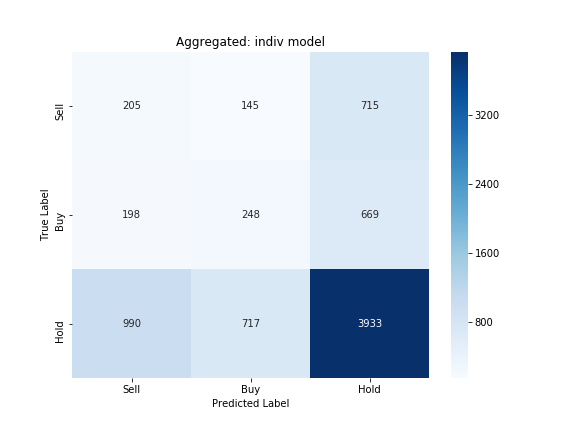
\includegraphics[width=.62\textwidth]{images/CMs/CM_indiv_aggreg.png}
    \caption{Confusion matrix of the asset-specific model results aggregated for all testing periods and assets}
    \label{fig:CMAggrI}
\end{figure}

\begin{figure}[H]
    \centering
    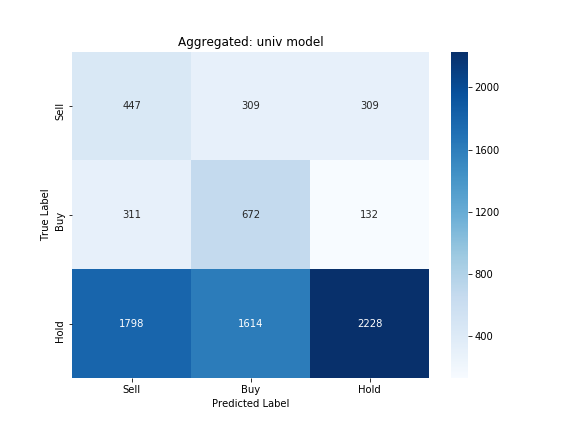
\includegraphics[width=.62\textwidth]{images/CMs/CM_univ_aggreg.png}
    \caption{Confusion matrix of the universal model results aggregated for all testing periods and assets}
    \label{fig:CMAggrU}
\end{figure}

As per Table \ref{tbl:ClassSign}, mean accuracy scores are significantly higher in case of the asset-specific model build, in each of the testing periods, at significance level $0.005$. In testing periods 1 and 3, the mean (macro) F1-score, precision and recall scores are all significantly higher in case of the universal model build at significance level $0.05$. In period 2, the mean F1-score, precision and recall are all significantly higher in case of the universal model at significance level $0.02$. 

\begin{table}[H]
\centering
\begin{tabular}{l|l|c}
 Test period & Metric    & \multicolumn{1}{c}{p-value (equal means)} \\ \hline \hline
 \multirow{4}{1cm}{2006-2007}  & Accuracy  & 0.003                  \\
 & F1-score   & 0.002                  \\
 & Precision & 0.002                  \\
 & Recall  & 0.003                  \\ \hline
 \multirow{4}{1cm}{2008-2009} & Accuracy  & 0.000                  \\
 & F1-score   & 0.017                  \\
 & Precision & 0.016                  \\
 & Recall  & 0.019                  \\ \hline
 \multirow{4}{1cm}{2017-2019} & Accuracy  & 0.001                  \\
 & F1-score   & 0.003                  \\
 & Precision & 0.002                  \\
 & Recall  & 0.004                 
\end{tabular}
\caption{Significance test: dependent Student's t-test on paired samples for classification scores. The null-hypothesis for each metric is that there is no significant difference in the mean scores of the asset-specific and universal model within each testing period.}
\label{tbl:ClassSign}
\end{table}

\subsection{Financial Performance}
\label{subsec:ER:FinPerf}

The annual returns and number of trades for each model, asset and period are displayed in Table \ref{tbl:FinResMain}. 

In terms of average annual returns, in the period before the crisis and the latest period starting in May 2017, the Buy\&Hold strategy brought the best results, but in the first period, this average is largely influenced by the outstanding annual price growth of the Apple stock. During the financial crisis (2008-2009) the universal model and the asset-specific model brought the highest and positive returns, though with the exception of Apple's stock, all prices decreased during the period. In most cases the universal model produced more annual returns than the individual model. In the first period, the asset-specific model, in the second, the RSI and in the third the two equally performed the worst. The universal model prompted the most trading activity, more than 8 times than the more traditional ones. The asset-specific model resulted in a lot of trades but on average it is still  49\% of that prompted by the universal. 

\begin{table}[H]
\begin{tabular}{l|l|ccccc|ccccc}
\multicolumn{1}{m{1cm}|}{\multirow{2}{1cm}{Test period}} & \multicolumn{1}{m{1.5cm}|}{\multirow{2}{1.5cm}{Tested Assets}} &       \multicolumn{5}{c|}{Annual Return} & \multicolumn{5}{c}{Number of trades} \\ \cline{3-12}
  &                  &  CNN-I         & CNN-U         & RSI           & BB            & B\&H          & CNN-I            & CNN-U & RSI & BB & B\&H \\ \hline \hline
\multirow{6}{1cm}{2006-2007} & S\&P500       & 0.07          & \textbf{0.13} & 0.06          & 0.08          & 0.07          & 52               & 89    & 7   & 12 & 2    \\
  & Nikkei225        &  0.00          & 0.05          & \textbf{0.08} & 0.07          & -0.03         & 44               & 94    & 9   & 11 & 2    \\
  & Nasdaq       & 0.01          & 0.07          & 0.05          & -0.01         & \textbf{0.08} & 37               & 92    & 7   & 7  & 2    \\
  & AAPL             & 0.27          & 0.18          & 0.32          & 0.35          & \textbf{0.63} & 38               & 72    & 10  & 10 & 2    \\
  & SPY              & 0.06          & \textbf{0.12} & 0.06          & 0.03          & 0.09          & 44               & 94    & 7   & 7  & 2    \\ 
  \cline{2-12}
  & \textit{Std.Dev.}  & 0.11 & 0.05 & 0.11 & 0.14 & 0.26 & 6 & 9 & 1 & 2 & 0    \\
  \cline{2-12}
  & \textit{Average}  & 0.08          & 0.11          & 0.11          & 0.10          & \textbf{0.17} & 43               & 88    & 8   & 9  & 2    \\ \hline
\multirow{6}{1cm}{2008-2009} & S\&P500           & 0.03 & \textbf{0.16} & -0.20 & -0.13 & -0.12 & 57 & 64 & 2 & 6  & 2 \\
 & Nikkei225         & 0.01 & \textbf{0.03} & -0.10 & -0.14 & -0.17 & 46 & 66 & 8 & 9  & 2 \\
 & Nasdaq            & 0.10 & \textbf{0.22} & -0.12 & 0.05  & -0.07 & 34 & 68 & 4 & 14 & 2 \\
 & AAPL              & \textbf{0.35} & 0.05 & -0.23 & -0.16 & 0.04  & 30 & 62 & 6 & 10 & 2 \\
 & SPY               & 0.03 & \textbf{0.33} & -0.19 & -0.16 & -0.10 & 37 & 78 & 2 & 6  & 2 \\ \cline{2-12} 
 & \textit{Std.Dev.} & 0.14 & 0.13 & 0.05  & 0.09  & 0.08  & 11 & 6  & 3 & 3  & 0 \\ \cline{2-12} 
 & \textit{Average}  & 0.10 & \textbf{0.16} & -0.17 & -0.11 & -0.08 & 41 & 68 & 4 & 9  & 2 \\ \hline
\multirow{6}{1cm}{2017-2019} & S\&P500       & 0.05          & 0.01          & -0.01         & \textbf{0.11} & 0.08          & 40               & 120   & 5   & 13 & 2    \\
  & Nikkei225     & 0.09          & \textbf{0.11} & 0.05          & 0.00          & 0.02          & 51               & 111   & 9   & 11 & 2    \\
  & Nasdaq         & 0.02          & 0.05          & 0.05          & 0.10          & \textbf{0.11} & 56               & 112   & 7   & 11 & 2    \\
  & AAPL      & 0.07          & 0.09          & \textbf{0.18} & -0.01         & 0.13          & 47               & 114   & 11  & 11 & 2    \\
  & SPY       & 0.04          & 0.06          & 0.00          & \textbf{0.11} & \textbf{0.11} & 49               & 116   & 5   & 13 & 2    \\ 
  \cline{2-12}
  & \textit{Std.Dev.}  & 0.03 & 0.04 & 0.08 & 0.06 & 0.04 & 6 & 4 & 3 & 1 & 0\\
  \cline{2-12}
  & \textit{Average} & 0.05          & 0.06          & 0.05          & 0.06          & \textbf{0.09} & 49               & 115   & 7   & 12 & 2   
\end{tabular}
\caption{Annual returns and Number of trades for the asset-specific model (CNN-I), the universal model (CNN-U) and the competing strategies: Relative Strength Index (RSI), Bollinger Bands (BB) and Buy\&Hold (B\&H)}
\label{tbl:FinResMain}
\end{table}

The significance test results for the annual returns are in Table \ref{tbl:AnnRes_Signf}. The mean annual returns are not significantly different for any of the strategy combinations in the first and last testing period. On the other hand, during the crisis (2008-2009), the annual returns produced by the asset-specific and the universal model build are significantly higher when matched against the other three competing strategies (at significance level $0.05$ except for the asset-specific model versus the BB strategy when the significance level is $0.1$). The annual returns are, however, not significantly different when comparing the asset-specific and universal models.

\begin{table}[H]
\centering
\begin{tabular}{l|l|l|c}
\multicolumn{1}{m{1cm}|}{\multirow{2}{1cm}{Test period}}  & \multicolumn{2}{c|}{Strategies}  & \multicolumn{1}{m{2cm}}{\multirow{2}{2cm}{p-value of equal means}} \\ \cline{2-3}
             & Strategy 1 & Strategy 2 &         \\ \hline \hline
\multirow{7}{1cm}{2006-2007}  & CNN-I      & CNN-U      & 0.41    \\
             & CNN-I      & RSI        & 0.12    \\
             & CNN-I      & BB         & 0.39    \\
             & CNN-I      & B\&H       & 0.28    \\
             & CNN-U      & RSI        & 0.91    \\
             & CNN-U      & BB         & 0.92    \\
             & CNN-U      & B\&H       & 0.58    \\ \hline
\multirow{7}{1cm}{2008-2009} & CNN-I      & CNN-U      & 0.62    \\
             & CNN-I      & RSI        & 0.03    \\
             & CNN-I      & BB         & 0.05    \\
             & CNN-I      & B\&H       & 0.00    \\
             & CNN-U      & RSI        & 0.01    \\
             & CNN-U      & BB         & 0.01    \\
             & CNN-U      & B\&H       & 0.03    \\ \hline
\multirow{7}{1cm}{2017-2019}  & CNN-I      & CNN-U      & 0.48    \\
             & CNN-I      & RSI        & 0.97    \\
             & CNN-I      & BB         & 0.85    \\
             & CNN-I      & B\&H       & 0.30    \\
             & CNN-U      & RSI        & 0.71    \\
             & CNN-U      & BB         & 0.95    \\
             & CNN-U      & B\&H       & 0.47   
\end{tabular}
\caption{Significance test: dependent Student’s t-test on paired samples of annual returns for each testing period. The null-hypothesis for each pair of strategies is that the mean annual return in a given period is equal}
\label{tbl:AnnRes_Signf}
\end{table}


Additional financial results about cumulative returns, total profit \& loss and average P\&L per trade can be seen in the Appendices.

\subsection{Time Consumption}
\label{subsec:ER:TimePerf}

The results of timing were calculated while running in Google Colaboratory using Google's Nvidia Tesla K80 GPU and 12GB of RAM.

The average training time of the asset-specific model in the first test period is 7 minutes and 6 seconds, which is $1/6$ of the universal model's 42 minutes and 9 seconds. 
In the second period, the universal model took 42 minutes and 35 seconds to train, 6.5 times longer than the asset-specific model, and in the third period, the universal model training only took 3.65 longer than the average 8 minutes and 27 seconds of the individual model training. These numbers depend on batch size, the number of images passed for training and model complexity.

The time to produce predictions for an image takes on average less in case of the universal model build but in each case both models come up with a prediction in less than a 1.5 milliseconds.

\begin{table}[H]
\centering
\begin{tabular}{l|l|cc|cc}
\multicolumn{1}{m{1cm}|}{\multirow{2}{1cm}{Test period}} & \multicolumn{1}{m{1.5cm}|}{\multirow{2}{1.5cm}{Tested Assets}} & \multicolumn{2}{c|}{Training time (mm:ss) } & \multicolumn{2}{c}{Testing time (ms/image)} \\ \cline{3-6}
&& CNN-I & CNN-U & CNN-I & CNN-U \\ 
\hline \hline
\multirow{6}{1cm}{2006-2007} & S\&P500   & 08:30 & 42:09 & 0.79 & 0.77 \\
          & Nikkei225 & 07:12 & 42:09 & 1.14 & 0.17 \\
          & Nasdaq    & 04:59 & 42:09 & 0.79 & 0.17 \\
          & AAPL      & 10:56 & 42:09 & 1.16 & 0.13 \\
          & SPY       & 03:53 & 42:09 & 1.21 & 0.17 \\ \cline{2-6}
          & \textit{Average}   & 07:06 & 42:09 & 1.02 & 0.29 \\ \hline
\multirow{6}{1cm}{2008-2009} & S\&P500          & 08:04 & 42:35 & 0.71 & 0.74 \\
 & Nikkei225        & 07:57 & 42:35 & 0.76 & 0.18 \\
 & Nasdaq           & 06:29 & 42:35 & 0.73 & 0.18 \\
 & AAPL             & 06:00 & 42:35 & 0.77 & 0.17 \\
 & SPY              & 04:09 & 42:35 & 0.73 & 0.19 \\ \cline{2-6} 
 & \textit{Average} & 06:32 & 42:35 & 0.74 & 0.29 \\\hline
\multirow{6}{1cm}{2017-2019} & S\&P500   & 15:33 & 31:00 & 0.63 & 0.59 \\
          & Nikkei225 & 08:34 & 31:00 & 0.57 & 0.11 \\
          & Nasdaq    & 06:41 & 31:00 & 0.55 & 0.15 \\
          & AAPL      & 05:52 & 31:00 & 0.59 & 0.13 \\
          & SPY       & 05:35 & 31:00 & 0.61 & 0.11 \\ \cline{2-6}
          & \textit{Average}   & 08:27 & 31:00 & 0.59 & 0.22
\end{tabular}
\caption{Training and testing times of asset-specific models (CNN-I) and universal models (CNN-U). Note, that the training times for the different assets in case of the universal model is the same as only one universal model is trained per period which is then used to return trading signal predictions on each asset's testing data per image on average.}
\label{tbl:TimeRes}
\end{table}

In Figure \ref{fig:imageCrea}, we can see how long it takes to create the three representations required for the prediction of a new trading signal upon observation of a new price. The figure shows execution times to transform a price series into a return series with $N$ elements and then create three $N \times N$ sized image representations of those, one RP, one GAF and one MTF with the parameters set as discussed in the section \nameref{sec:DM}. Our model uses $30 \times 30$ images, so in our case on average it takes $3.59$ milliseconds to make new inputs. 

\begin{figure}[h]
    \centering
    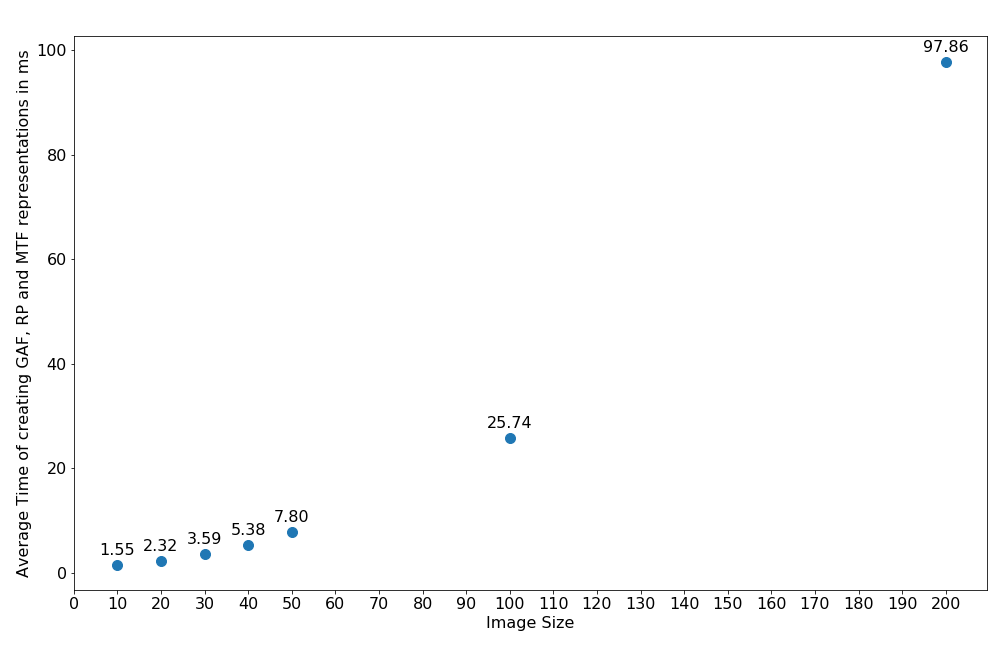
\includegraphics[width=\textwidth]{images/Image_Trf_Times.png}
    \caption{The plot shows the number of milliseconds it takes on average to turn a price series into a return series and create three image representations (RP, GAF and MTF).}
    \label{fig:imageCrea}
\end{figure}

\section{Discussion}
\label{sec:Discuss}

\subsection{Asset-specific models \& Universal models}

We note, that the two model builds are not only differing in the data used for training but as per best practice in building a deep learning model, further tuning was carried out to obtain the highest possible performance of the model. As discussed before, these differences are reflected in mini batch sizes, regularization and optimization hyper-parameters, and class weights applied on the loss function.

To determine the differences between the two model builds, we will firstly concentrate on the classification results. We saw in Table \ref{tbl:ClassSign} and \ref{tbl:ClassRes}, that mean accuracy is higher in case of the asset-specific model builds. Since accuracy is adding up the diagonal of the confusion matrix, and then dividing it with the sum of all elements of the confusion matrix, the reason for the difference in accuracy is clear when comparing the diagonal of Figure \ref{fig:CMAggrI} and Figure \ref{fig:CMAggrU}. The asset-specific model predicts much more of the "Hold" labelled images as "Hold" than the universal build, which in turn classifies much more of the "Buy" and "Sell" images correctly, but not enough to offset the misclassified "Hold" images which results in the lower accuracy. All of the macro F1, precision and recall scores provide us with a better tool to examine the results of classification when we are interested in the complete picture and not the overpowering effect of the successful prediction of one class. These scores are significantly higher in case of the universal model build (even in testing period 2 where these measurements are lower) and this result is due to the macro averages being dragged down by the poor rate of correct classifications of the "Buy" and "Sell" images, as shown in the \nameref{subsec:ER:ClassPerf} section. We should note, that the achieved classification results should be further enhanced by changing the network architecture, by altering the input or using other tools, however, the time constraint allowed for the presented results.

But what drives these differences between the models? Firstly, the weights applied on the loss function to fight class imbalance have an impact on the distribution of the predicted classes. Furthermore, the underlying data for the training of the two model types differs in characteristics and size which is then naturally reflected in the results. 

In our case, we should of course seek many correct predictions for each of the classes, but for trading purposes, we are less interested in predicting many correct "Hold"-s, and more inclined to find the points where we should make a move. This might be dependent on the asset price's movements and fluctuations, or the attitude of the investor but in most cases it is more important to classify lots of "Sell" and "Buy" points correctly. 
We can think about this by observing that, often the incorrect classifications of these two classes only represent a missed opportunity to trade: when they are predicted to be “Hold”, or when the earlier mentioned safety feature prevents order-execution. The downside to this is the increase in the number of misclassified “Hold” points. If the safety feature does not prevent against execution of a "Buy" or "Sell" prediction at a price that should be associated with a "Hold", we experience trades that, to some extent, eliminate the positive effect of the correct predictions. For example, by executing a false “Buy” order in place of a “Hold”, the algorithm prohibits the execution of the correctly predicted “Buy” a couple time steps later. 

To see how the two strategies differ, we move on to the comparison of financial performance.
\begin{figure}[ht]
    \centering
    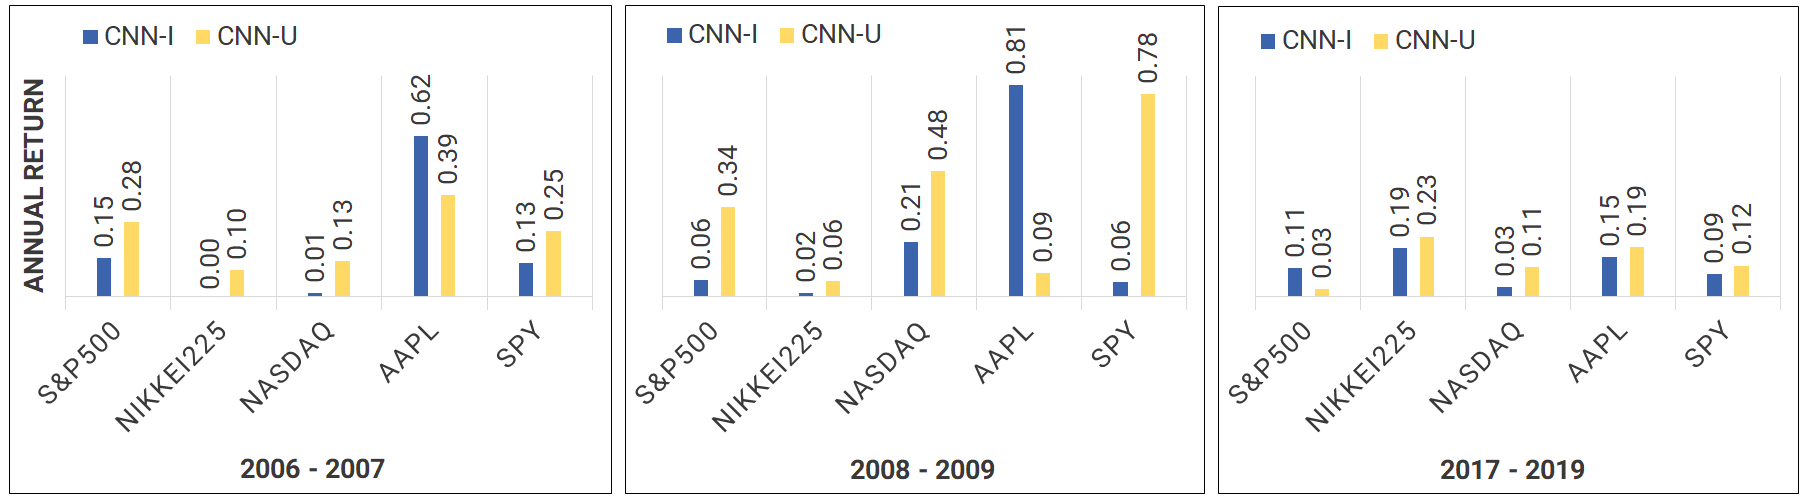
\includegraphics[width=\textwidth]{images/CNNIvsCNNU.png}
    \caption{Comparison of annual returns of the asset-specific model (CNN-I) and the universal model (CNN-U) for each testing period and asset.}
    \label{fig:CNNIvsCNNU}
\end{figure}
Though there are no significant differences in the mean annual returns of the asset-specific and universal models, the universal model produced higher annual returns in 12 out of 15 cases. 
Figure \ref{fig:CNNIvsCNNU} shows that the three exceptions are the Apple stock in both the first and second period, and in the third period, the annual return was a bit higher using the model trained on the S\&P500 data exclusively, than using the universal set. We also see that the universal model on average executes more than two times as many trades as the asset-specific model, which is due to the higher number of “Buy” and “Sell” predictions. 
In Figure \ref{fig:AAPLcapevol} we see the positive effect of a larger number of correct “Hold” predictions, on the cost of less “Buy” and “Sell”, as in case of the asset-specific model.
Moreover, we use Figure \ref{fig:SPYcapevol} to point out why, in some cases, it is worth to have more “Buy” and “Sell” predictions, correct and incorrect as well, as in case of the universal model. 
The capital evolution plot when trading the AAPL stock according to the different trading strategies during 2008-2009 shows an example when the asset-specific model clearly performs great financially as opposed to any of the other strategies. The periods of constant capital signifies times when the capital is hold in cash, while periods of following the price movements of the asset (purple B\&H line) signifies periods of holding the instrument. Now, one distinguishing aspect of the blue line in Figure \ref{fig:AAPLcapevol}, showing the capital changes according to the trade orders of the asset-specific model, to the yellow line (denoting the same for the universal model) is that the asset-specific model keeps the asset-form for longer periods of time, while the universal model only does that for shorter periods. 
The advances from keeping the asset for longer periods appear during March 2008 - May 2008 and for briefer periods in November 2008 and March 2009. These were periods where the universal model failed to avoid selling the asset prematurely which might be due to the many false predictions of "Sell". Now we are turning to Figure \ref{fig:SPYcapevol} which shows the capital evolution for the same period but trading the SPDR S\&P500 ETF instances. 
Contrary to the previous, here the universal model provides higher returns (path marked by the yellow line) which proved fruitful during e.g. the periods August 2008 - October 2008 and March 2009. Since many of the trading opportunities were missed due to the lack of predicted "Buy" and "Sell" orders, the asset-specific model was taken by the downward stream of the market (though it still managed to perform better). 
It is worth to note, that, during the periods of keeping cash, one could utilize the money in different ways such that further probable gains are acquired from trading other instruments or investing in the risk-free asset (if it gives positive returns). This could boost the trader's income while employing the universal model. 

Overall, both the asset-specific and universal model builds have their benefits and flaws and both could use further tuning to encourage better classification performance. However, the universal model seem to perform slightly better in almost all cases and finds more of the trading points correctly, thus we deem that to be a bit better. Also, in case of a similar performance, model training takes longer for the universal model, but training just one model, with the prices of many assets of various types would make this model more robustly useful for a trader. 
For example, if a trader decides to return predictions for a new asset, in case of the asset-specific model, a whole newly tuned model building and training is required. On the other hand, if the newly traded asset is part of the universal model build, there is no need for retraining, the universal model can be readily used.
\begin{figure}[H]
    \centering
    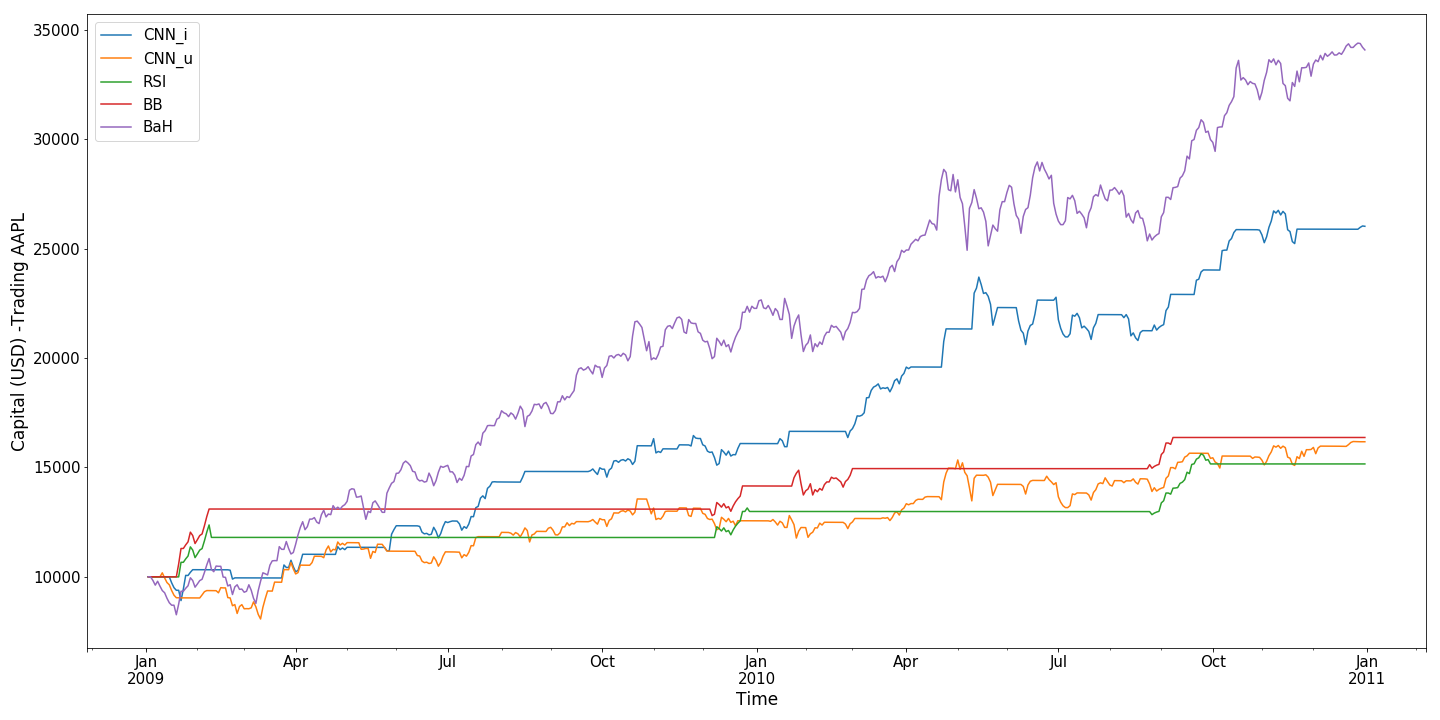
\includegraphics[width=\textwidth]{images/capitals/Capitals2_AAPL.png}
    \caption{The evolution of the capital (initial capital is \$ 10,000) during 2008-2009 trading the AAPL stock according to the different trading strategies: asset-specific model (CNN-i), universal model (CNN-u), RSI, BB and Buy\&Hold (B\&H)}
    \label{fig:AAPLcapevol}
\end{figure}
\begin{figure}[H]
    \centering
    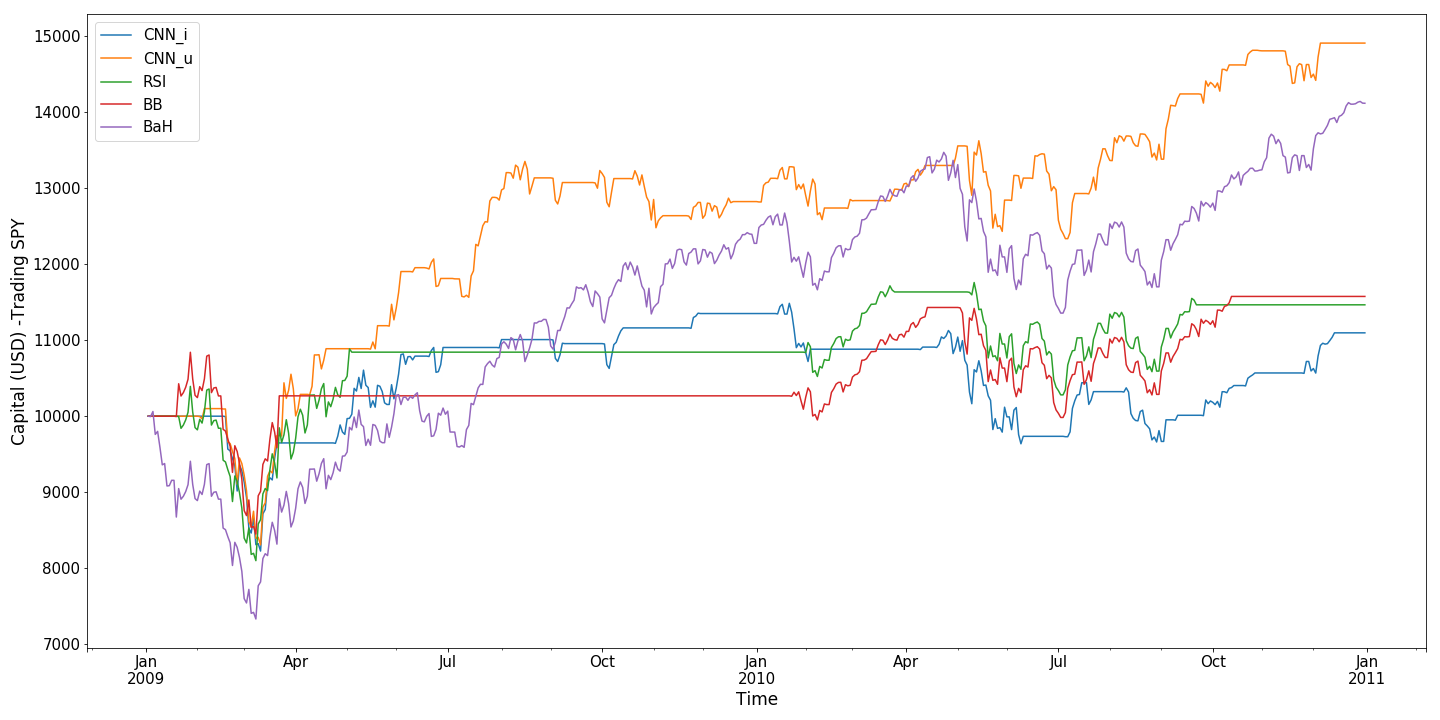
\includegraphics[width=\textwidth]{images/capitals/Capitals2_SPY.png}
    \caption{The evolution of the capital (initial capital is \$ 10,000) during 2008-2009 trading the SPY according to the different trading strategies: asset-specific model (CNN-i), universal model (CNN-u), RSI, BB and Buy\&Hold (B\&H)}
    \label{fig:SPYcapevol}
\end{figure}


\subsection{Competing algorithmic strategies \& the CNN}

The main metric to determine performance of the different strategies is annual return. 
To recap, we compare the financial profitability of the CNN-I (asset-specific model) and the CNN-U (universal model), with two traditional strategies: the RSI (relative strength index) and the BB (Bollinger Bands), and a simple market following strategy, the B\&H (Buy\&Hold). 
Table \ref{tbl:FinResMain} shows the annual returns in each testing period for each asset, and from Table \ref{tbl:AnnRes_Signf} we know, that the differences in mean annual returns as opposed to the traditional and B\&H strategies were only significant in the period 2008-2009. 
These results indicate that the CNN models generally perform similarly good as the other strategies during economic regimes with increasing prices. However, during a period of falling prices, such as the financial crisis, when the traditional strategies fail to generate income, the CNN still makes for positive returns. 
Figure \ref{fig:CNNvsComp_2} shows these returns for the different strategies and testing assets. The lowest returns were acquired during the trading of the Nikkei225, but it is still a high profit considering that its price fall on average 17\% annually during the period. As we can see in Figure \ref{fig:N225capevol}, up to October 2008, the trading with the RSI strategy ensured some profits but then failed to sell before the further fall in price and so it stayed in the negative zone. The two CNN models behaved very similarly. 
Except for some brief periods in 2009, the universal setting managed to find more of the timely "Buy" and "Sell" points than the asset-specific one. Despite both CNN models failed to sell just before October 2008, they could still save the capital with some well-timed orders in October 2008.
\begin{figure}[ht]
    \centering
    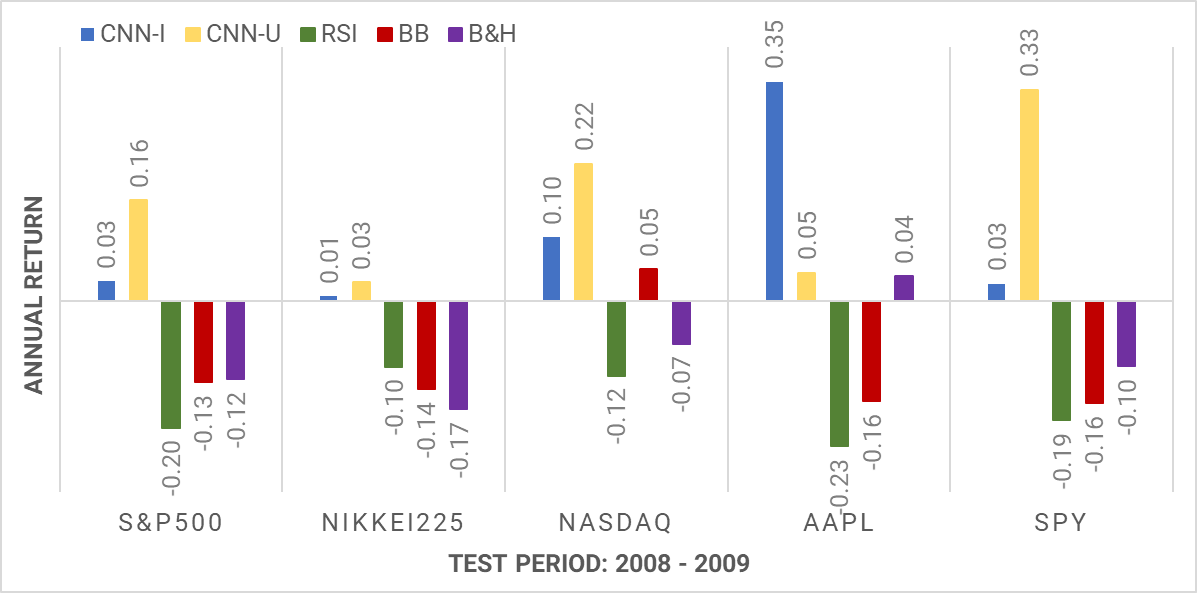
\includegraphics[width=.75\textwidth]{images/CNNvsComp_Crisis.png}
    \caption{Annual returns after trading different assets during the financial crisis (test period 2) according to the strategies: asset-specific model (CNN-I), universal model (CNN-U), RSI, BB and Buy\&Hold (B\&H)}
    \label{fig:CNNvsComp_2}
\end{figure}

\begin{figure}[ht]
    \centering
    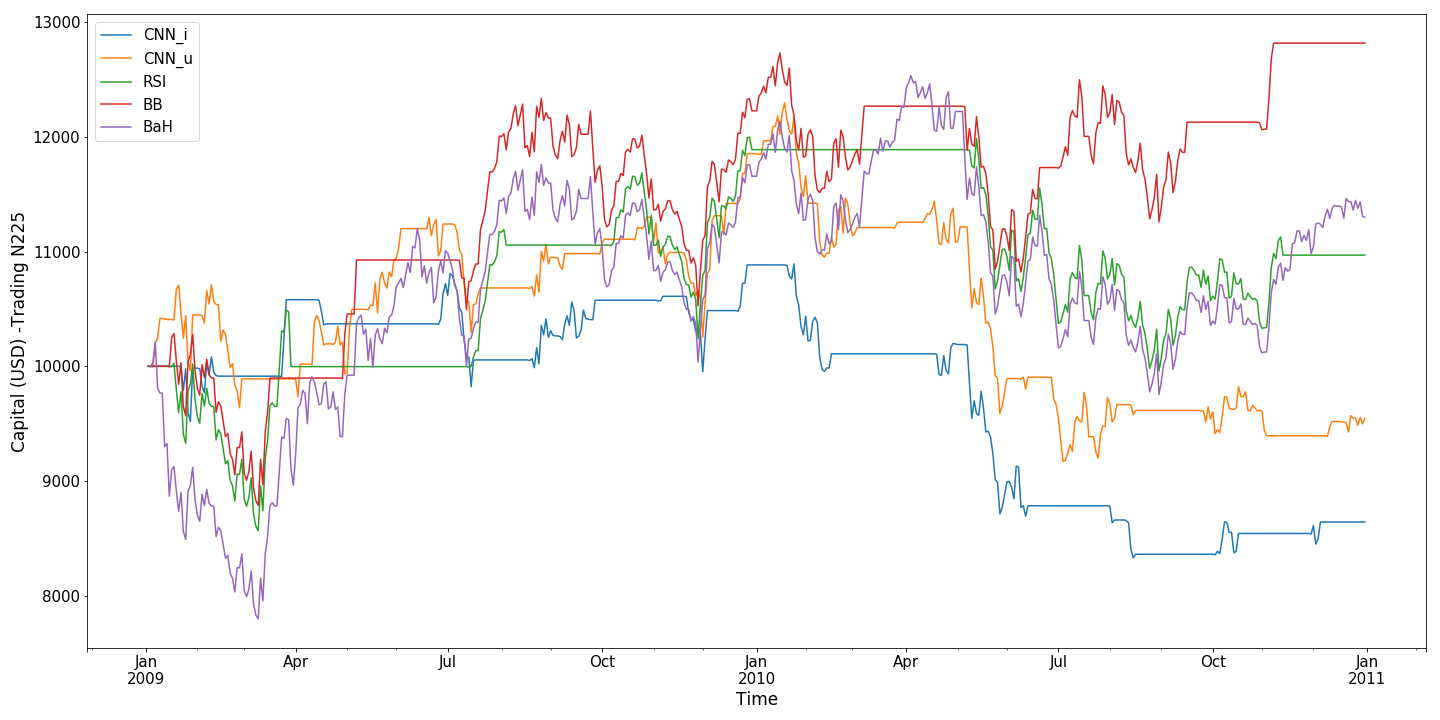
\includegraphics[width=\textwidth]{images/capitals/Capitals2_N225.png}
    \caption{The evolution of the capital (initial capital is \$ 10,000) during 2008-2009 trading the Nikkei225 according to the different trading strategies: asset-specific model (CNN-i), universal model (CNN-u), RSI, BB and Buy\&Hold (B\&H)}
    \label{fig:N225capevol}
\end{figure}

Moving on to testing period 1, we can see in the left plot in Figure \ref{fig:CNNvsComp_P1P3} that the trades initiated by the CNN-U model brought higher profits than any other strategy in case of the S\&P500 and the SPY. It also brought positive profits when trading the Nikkei225, when the price was actually falling, but could not score above the RSI and the BB strategies. The CNN also performed relatively poor when the price of the AAPL stock was soaring (63\% annually on average). 

In Figure \ref{fig:P1_AAPLcapevol}, we can see that the CNN-U model did not quite manage to find the timely trading points and only provided capital above the B\&H during June 2006 - September 2006 when the stock price was decreasing a bit. The trading strategy dictated by the CNN-I was quite successful up until May 2007. After that point the stock price started fluctuating quite a lot and increased much faster than in the previous part of the period and the CNN could not keep up with this change in the distribution. 

\begin{figure}[H]
    \centering
    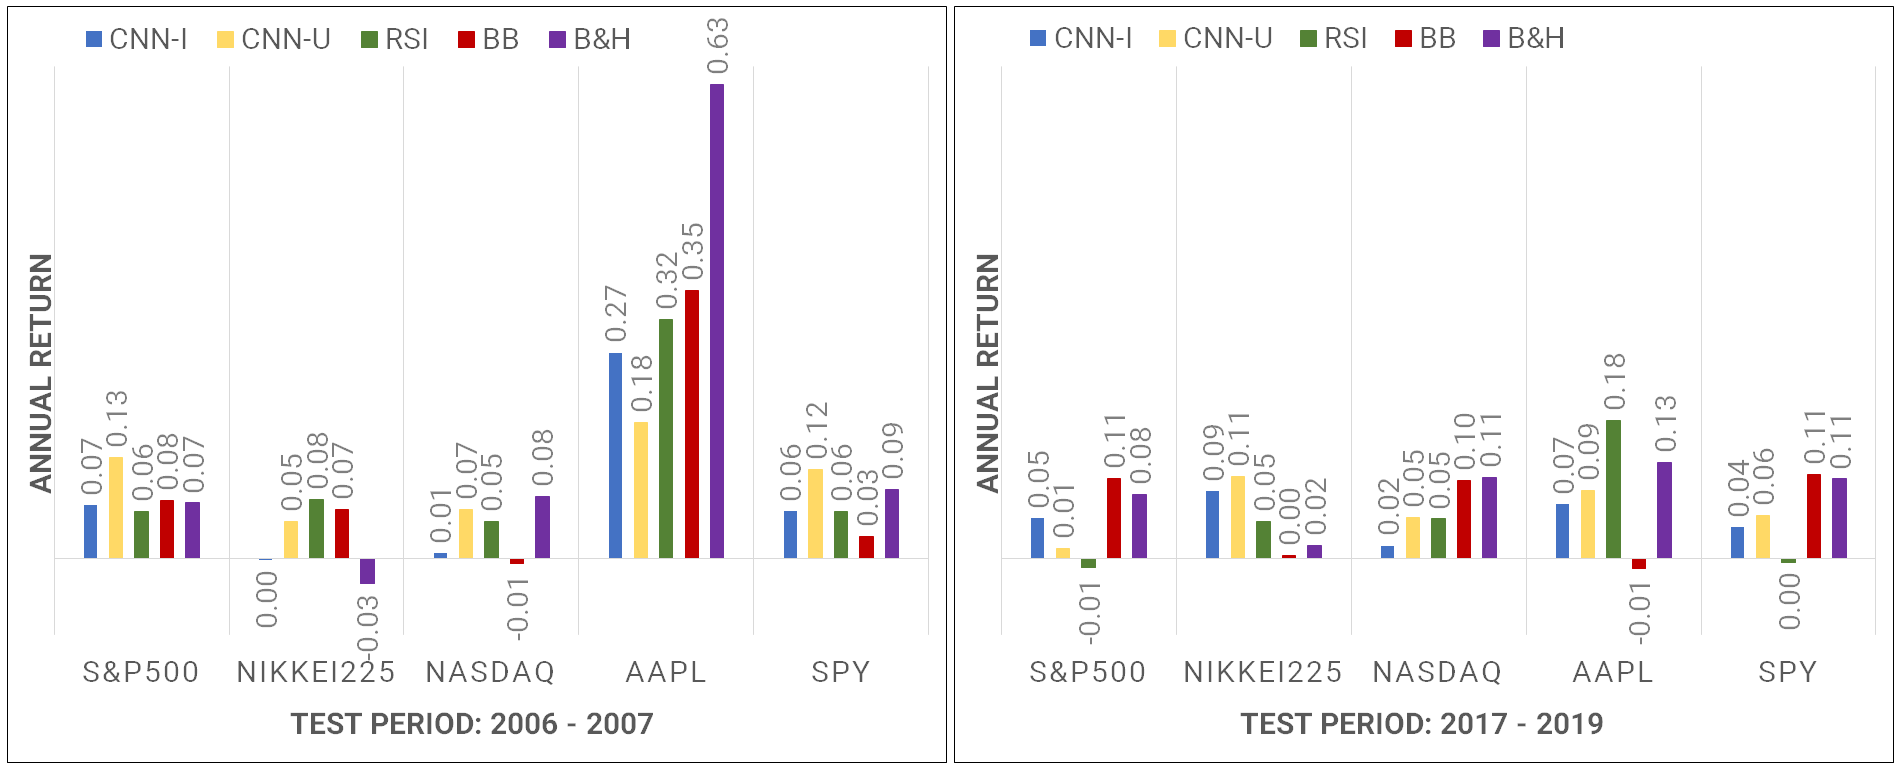
\includegraphics[width=\textwidth]{images/CNNvsComp_P1P3.png}
    \caption{Annual returns after trading different assets during test periods 1 (2007-2007) and 2 (May 2017 - June 2019) according to the strategies: asset-specific model (CNN-I), universal model (CNN-U), RSI, BB and Buy\&Hold (B\&H)}
    \label{fig:CNNvsComp_P1P3}
\end{figure}

\begin{figure}[H]
    \centering
    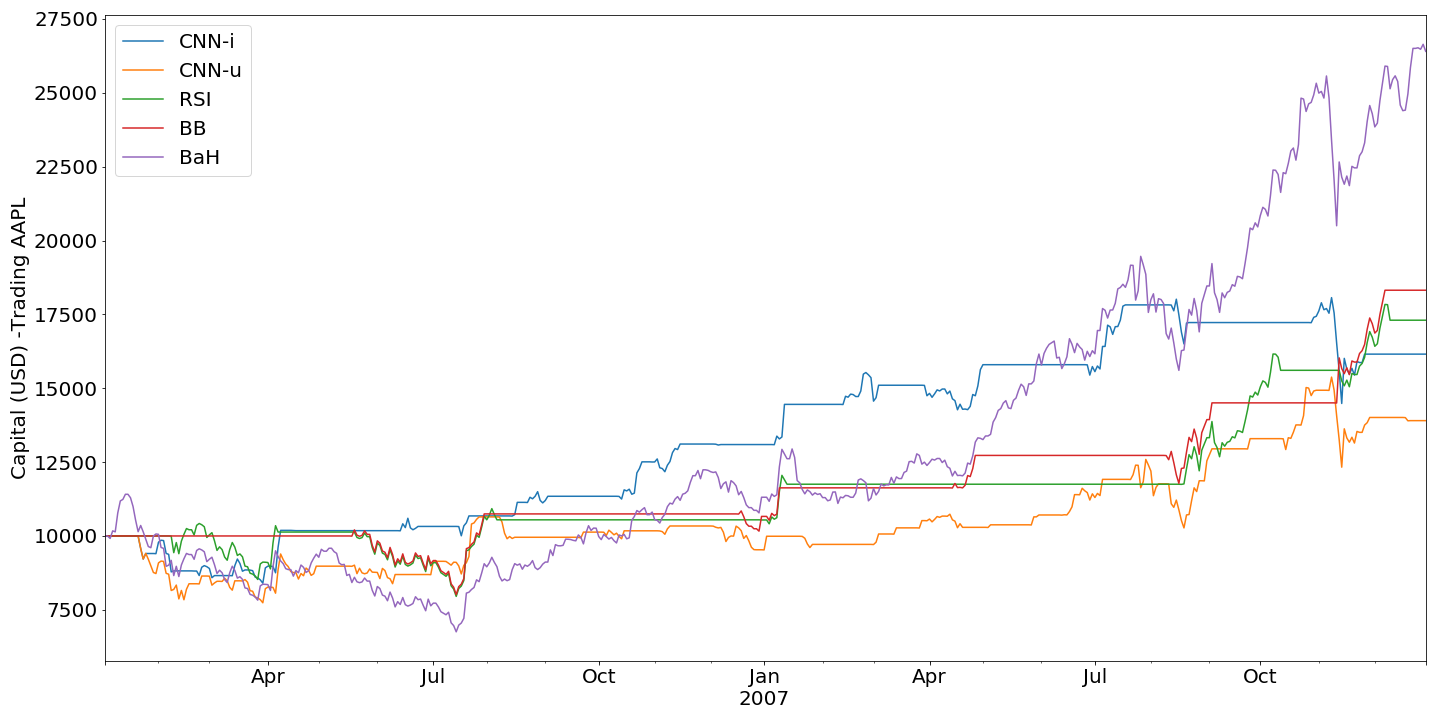
\includegraphics[width=\textwidth]{images/capitals/Capitals1_AAPL.png}
    \caption{The evolution of the capital (initial capital is \$ 10,000) during 2006-2007 trading the Apple stock according to the different trading strategies: asset-specific model (CNN-i), universal model (CNN-u), RSI, BB and Buy\&Hold (B\&H)}
    \label{fig:P1_AAPLcapevol}
\end{figure}

In the latest period of May 2017 - June 2019, the market is similar to that in the first period but with slightly higher returns. The exception is the Apple stock which did not see such a growth lately as 10 years earlier. Although there is no significant difference between the mean annual returns during this period, the CNN models showed a weaker performance. The expectation was that the models would prove more successful due to the larger amount of past data that can be used to train the model. 
This was reflected in the slightly improved classification results in testing period 3 but not so much in the financial results. The Nikkei225 was the only asset that was traded more profitably by the CNN models than the competing strategies.

In Figure \ref{fig:P3_N225capevol} we can observe that the capital handled by the CNNs was vastly following the asset price from March 2018 with shorter periods of keeping cash. Then, between December 2018 and January 2019 both CNN models manage to sell the assets just before the price plunges and make great gains on the increase during the rest of 2019. The RSI and BB lead capitals both followed the plunge and lost a lot of it in doing so. 
The path of the capital when the SPY is traded during the third period in Figure \ref{fig:P3_SPYcapevol} shows an example where both CNN models failed to predict a "Sell" sign before the prices dropped in December 2018 - January 2019. Though the BB (green line) buys the asset when the price drops by a lot (passing the lower BB), when the prices keep falling, it never sells until the price starts increasing again. Now, if the price increases and quick enough, the trader just loses a lot without actually waiting for the price to grow again and initiate the sell then. A typical case of this is trading the SPY ETF between February 2018 and June 2018 or between October 2018 and February 2019. 
The CNN models make a similar mistake in the second mentioned period: they both fail to make profits on the fluctuations starting in October 2018, and then, when the price drops, they both hold the asset and lose a lot of the built up capital. Afterwards, the CNN-I sells during the first two month of 2019 and thus misses out on the increasing market. The CNN-U also sells in January 2019 but keeps buying and selling, making some steps upwards. The RSI however done a good job in following the market price and at times moving above the Buy\&Hold capital. A plausible reason why the CNN model made profits over other strategies during this plunge during December 2018 - February 2019 in case of the N225 is that there was a clear-cut peak just before it. There, the model found a selling point and since the price quickly corrected back, there was not enough time for a "Buy" order to ruin the earnings. However, the price of the SPY did not just fall from a peaky point but had multiple small local maximums afterwards. The CNN-U bought into SPY at the second one, while the CNN-I at the third. This might be an issue that can be fixed by increasing the window of prices when we label the images, but such a change might also result in missed opportunities elsewhere. It is also worth to note, that the CNN models perform a very active trading strategy when compared with the other strategies.
\begin{figure}[H]
    \centering
    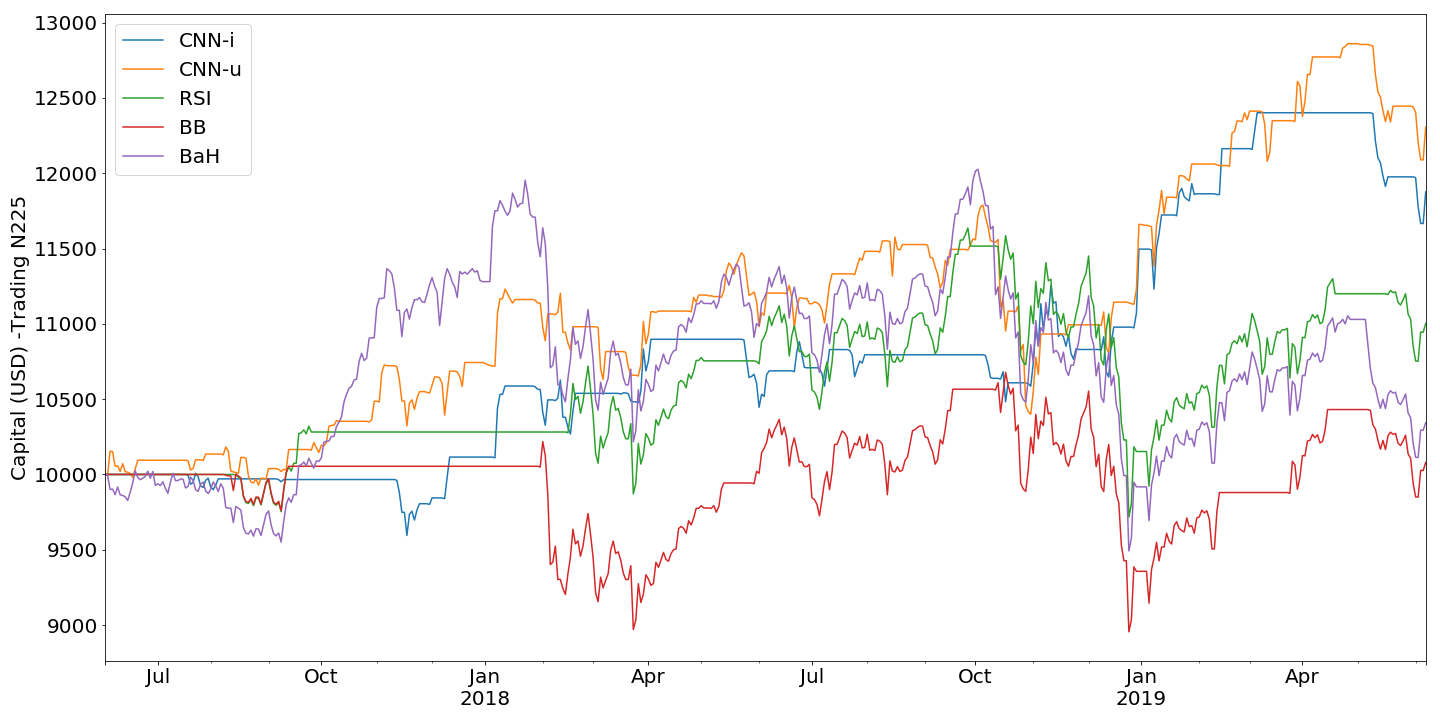
\includegraphics[width=.99\textwidth]{images/capitals/Capitals3_N225.png}
    \caption{The evolution of the capital (initial capital is \$ 10,000) during 2017-2019 trading the Nikkei225 according to the different trading strategies: asset-specific model (CNN-i), universal model (CNN-u), RSI, BB and Buy\&Hold (B\&H)}
    \label{fig:P3_N225capevol}
\end{figure}
\begin{figure}[H]
    \centering
    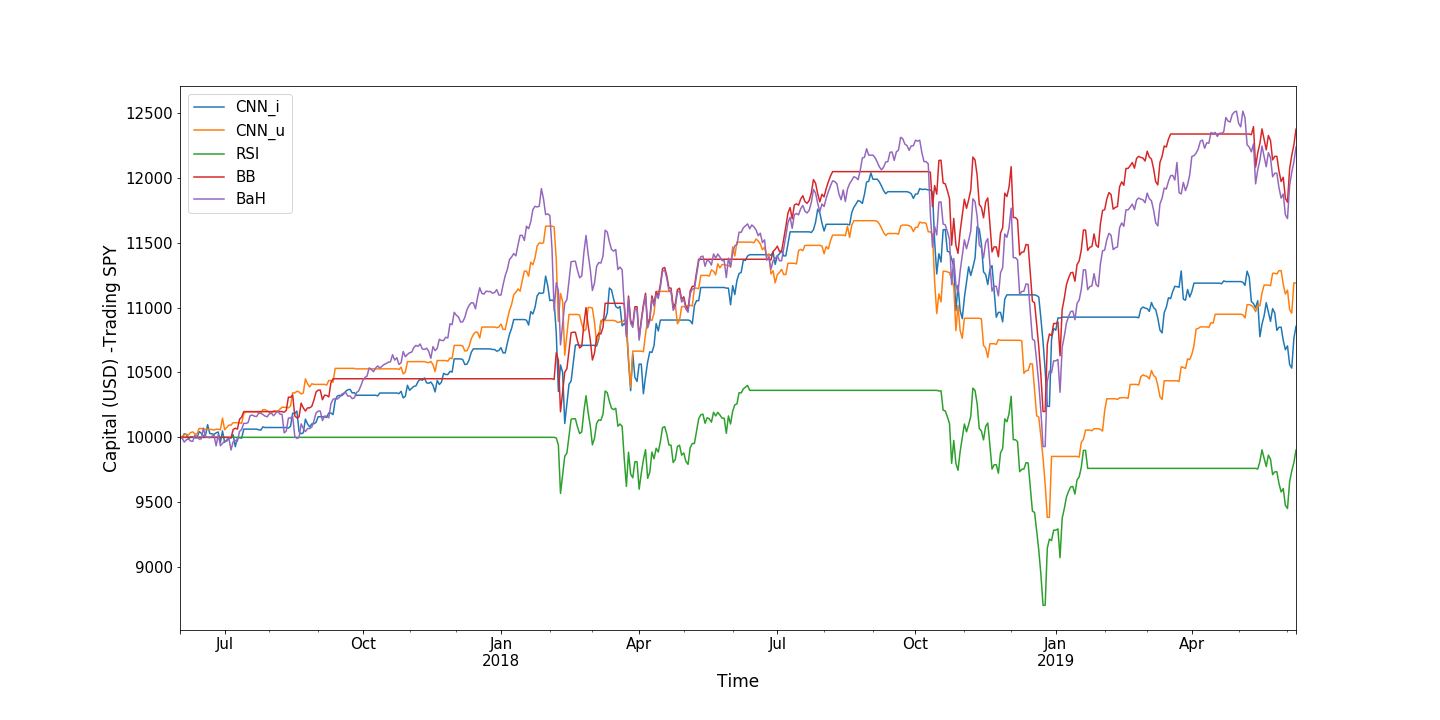
\includegraphics[width=.99\textwidth]{images/capitals/Capitals3_SPY.png}
    \caption{The evolution of the capital (initial capital is \$ 10,000) during 2017-2019 trading the SPDR S\&P500 ETF according to the different trading strategies: asset-specific model (CNN-i), universal model (CNN-u), RSI, BB and Buy\&Hold (B\&H)}
    \label{fig:P3_SPYcapevol}
\end{figure}
To sum up, the CNN models perform similarly to more traditional strategies and the Buy\&Hold given a growing market, but during a crisis with longer periods of low prices and some extreme fluctuations, the automatic trading models based on the CNN can outperform the competing strategies by quite a lot in profitability. The development of classification performance should further increase the expedience of the model, bringing in further profits. 

\subsection{Applicability based on execution times}

Overall, looking at the training/prediction times in Table \ref{tbl:TimeRes}, both CNN model variants are feasible to train and use for prediction as a real world trading application. The training of the asset-specific models take on average less than 10 minutes and the universal model training times are also below 45 minutes. These periods can easily fit into the time when the markets are closed and can further be decreased given more computational capacity (stronger GPU or TPU). The universal model training takes longer due to the larger amount of training images but in that case we only have to train one model which we can then use for the prediction of trading signals for multiple assets, not just one.
Moreover, in our tests we used a model for two years worth of predictions and the results are still promising which suggests that retraining of the model does not have to take place on a daily basis. 

The prediction time is quick enough even for intraday trading purposes. This is true even if we add the $3.59$ ms input creation time (see Figure \ref{fig:imageCrea}) to these prediction times so we know how long it takes for the model to return a trade signal given it observes a new price. To be more concise with the current input and model settings, for the asset-specific model, it takes maximum $4.8$ ($=1.21 + 3.59$) milliseconds, and for the universal model, a maximum of $4.36$ ($=0.77 + 3.59$) milliseconds to return a prediction. This means that given there is no further delay in observing the price and/or in executing a trading order getting it, one could trade on a five-millisecond frequency. Of course, on top of this we should add server call times and time of order execution, but the model can provide trading orders swift enough for high-frequency trading.

\section{Conclusion}
\label{sec:Conclusion}

The goal, to build a compact model, based on the CNN structure, which turns time series into images and predicts whether the trader should buy, sell or hold the asset at the latest price, is accomplished. The description in the \nameref{sec:DM} section and the code linked in the \nameref{app:GIT} section of the Appendix (\textbf{Lasse, Kenneth, Can I make my repository public on GitHub, or would that be against the contract with EY?}) makes the model and its components reproducible and ready for automation. 
Both the universal and asset-specific builds are capable of capturing the "Buy" and "Sell" patterns to an extent that the annual returns obtained using either one of them is not significantly different from those obtained by the proposed other strategies (RSI, BB, Buy\&Hold) during times when the market has an upward tendency.
The results also prove that within the boundaries of this experiment, both the CNN-I and CNN-U models beat the mentioned competing strategies during an economic regime with declining prices, such as the 2008 financial crisis. 
Although the classification performance has room for improvement, the additional progress would potentially make the trading strategy dictated by the model more successful than competing ones, even during a period of increasing prices. 

We also managed to compare the universal and asset-specific model structures, and the results seem to further support those found by \cite{sirignano2018universal}. While the asset-specific model showed better accuracy scores, it was due to the overwhelming prediction of "Hold" classes. 
When it comes to more balanced measurements of classification performance across all three classes, like the F1, precision and recall scores, the universal model achieved significantly higher values. It is also more robust in the sense, that one model can be used with the same settings over distinct asset classes and even more data would potentially further enhance the outcome. In spite of the fact that there is no statistically significant difference between the annual return results of the CNN-I and CNN-U models, the CNN-U model generally attained slightly higher returns. 

There are a lot of different ways to carry on investigating the introduced model. To explore the potential of the idea, however, there is a need for sufficient time and computational resources. Below, we cover the most relevant ways this model could be improved given ample resources.

For further enhancement of model performance, the model tuning could be carried out on a larger range of hyperparameters and model components. This further tuning would be more reliable if each model build would be validated multiple times on varying subsets of data, so the results are not dependent on the choice of the data instances in the validation set. There is a potential that the state-of-the-art CNN architectures, such as the VGG16 model by \cite{simonyan2014very}, the Inception-ResNet model by \cite{szegedy2016inception}, or the NASNet by \cite{zoph2018learning}, could also be used for this model, further enhancing the results.

In a real world scenario, a more rigorous testing of the model would be required before accepting the results and putting the model into production. Similarly as during training, each model build should be trained and tested multiple times on different subsets of the test data to ensure unbiased evaluation of the model performance.

To enable asymptotic significance testing when matching the performance against other strategies, it would make sense to test the model on more assets and look at different economic regimes to see how the model performs against e.g. a Buy \& Hold strategy in a market with decreasing prices. A further potential feature would be setting class weights dynamically, either in a rule-based setting or using a sort of regression model. For example, if an external indicator of market conditions suggests a bear market and the traders would want a more selling-heavy behaviour in such a market, they can set up a rule that changes the weights of the loss function, so that more "Sell" signals are produced than normally. Note, that this dynamic change can be generalized for the entire model, thus we can optimize a model for specific market conditions or risk-aversion levels and set up an algorithm to switch between the pre-trained models.

We mentioned previously, that the model is trained once, before testing it on an entire two year of data. It would make sense to test if the model produces better results with a more frequent retraining plan, especially if it is used for intraday training. This leads to the next point which is about the model making profit by trading a lot but turning smaller profits per trade (see Table \ref{tbl:PandLAvg}), as opposed to the competing strategies. This resembles the trading patterns of high-frequency trading strategies, which might indicate that the model could be successful in that domain.

Another option would be changing the assumptions of the model and use training images as if they were frames in a video where we wish to catch a pattern. This means that we would assume that the images are in fact dependent on each other on the time domain. Such an assumption would imply that the use of a recurrent neural network (RNN) or a long-short term memory network (LSTM) could be used to learn these dependencies in the data. Then, we could connect this model with the CNN and use the two models together to enhance each other's performance. Further investigation would be required to work out the architecture of this network and find out how the integration is feasible to serve the purpose of automatic trading. Similar use cases in the literature include emotion recognition in videos such as \cite{ebrahimi2015recurrent}.

Some of the general elements that could see further experimentation are the labelling and image creation methodology. It would be an option to alter the labels from "Buy", "Hold", "Sell" to a more granular version, e.g.: "Buy", "Weak-Buy", "Sell", "Weak-Sell", "Hold", thereby marking points leading up to a "Sell"/"Buy" signal that might be misinterpreted by the model. This would also ease the issue of label imbalance. Image creation can happen in various ways and the introduced transformation strategies can be modified or switched out entirely by other approaches. Besides using technical indicators as in \cite{sezer2018algorithmic}, more and more novel approaches appear in the literature \cite{sezer2019financial}.

The overall conclusion is that the proposed model, with the idea of using multiple time series to image transformation strategies, can compete with traditional strategies in the market in its current form. There are, however, multiple approaches to make improvements to this model, which could then lead to a more broad success of the idea.

\section{Appendices}
\label{sec:App}

\subsection{Code}
\label{app:GIT}
All relevant code and data is available in the following public GitHub repository: URL

\subsection{Gramian Angular Field: penalized inner product}
\label{app:GAF}
\begin{equation}
    \begin{split}
        \cos(\phi_1 + \phi_2)  & = \cos(\arccos(x) + \arccos(y)) \\
        & = \cos(\arccos(x)) \cdot \cos(\arccos(y)) - \sin(\arccos(x)) \cdot \sin(\arccos(y))\\
        & = x\cdot y - \sqrt{1-x^2} \cdot \sqrt{1-y^2}\\
        & = \langle x, y \rangle - \sqrt{1-x^2} \cdot \sqrt{1-y^2}
    \end{split}
\end{equation}
 Notice, that the entire operation does not satisfy the assumptions of an inner product (linearity limitation, not necessarily positive definite).

\subsection{Competing Strategies Description}
\label{app:CompetingStrats}

\subsubsection{Buy \& Hold}
The Buy \& Hold strategy is a simple and passive strategy based on buying an asset and keeping it for a long period of time, hoping for long term returns regardless of short term fluctuations on the market.
This will be represented in the testing periods as a Buy order on the first date and a Sell order on the last date with no other trades executed in between.

\subsubsection{Relative Strength Index}
The RSI (\cite{wilder1986relative}) is a momentum oscillator $[0, 100]$ with values over 70 indicating an overbought and below 30 and oversold asset. A Buy order happens when the RSI rises above 30 from below and a Sell is indicated by decreasing below 70 from above. The metric is defined by the two step calculation for a look-back period of $d=20$ days:
\begin{equation}
    \label{eq:RSI1}
    RSI_{step1} = 100 - \left[ \frac{100}{1 + \frac{Avg_d Gain}{Avg_d Loss}}\right]
\end{equation}
where $Avg_d Gain$ and $Avg_d Loss$ are the average percentage gains and/or losses during a look-back period of length $d$. After the first $d$ periods of data is available, the second step is just the smoothing of the step 1 formula:
\begin{equation}
    \label{eq:RSI2}
    RSI_{step2} = 100 - \left[ \frac{100}{1 + \frac{Previous Avg_d Gain \cdot (d-1) + Current Gain}{Previous Avg_d Loss \cdot (d-1) + Current Loss}}\right].
\end{equation}

\subsubsection{Bollinger Bands}
The Bollinger Bands (BB) (\cite{bollinger2002bollinger}) characterize the prices and the volatility of a financial asset. They can be depicted on the chart of an asset as a graphical band showing the envelope maximum and minimum of moving averages over the look- back period $d=20$, and the volatility is represented by the width of the envelope.
If the $d$-period moving average is given by $MA_d$, the $d$-period standard deviation is given by $\sigma_d$ and $c=2$ is a customizable parameter then the bands are:
\begin{equation}
    \label{eq:BBlow}
    lowerBB = MA_d - c \sigma_d
\end{equation}
and
\begin{equation}
    \label{eq:BBup}
    upperBB = MA_d + c \sigma_d.
\end{equation}
The strategy is to Buy when the Adjusted Close price decreases below the $lowerBB$ and Sell if it increases above the $upperBB$.

\subsection{Additional Financial Results}

\begin{table}[H]
\centering
\begin{tabular}{l|l|ccccc}
\multicolumn{1}{m{1cm}|}{\multirow{2}{1cm}{Test period}} & \multicolumn{1}{m{1.5cm}|}{\multirow{2}{1.5cm}{Tested Assets}} &       \multicolumn{5}{c}{Cumulative Return}  \\ \cline{3-7}
  &                  &  CNN-I         & CNN-U         & RSI           & BB            & B\&H \\ \hline \hline
\multirow{6}{1cm}{2006-2007}  & S\&P500          & 0.15              & \textbf{0.28} & 0.13          & 0.16          & 0.15          \\
  & Nikkei225        & 0.00              & 0.10          & \textbf{0.16} & 0.13          & -0.07         \\
  & Nasdaq           & 0.01              & \textbf{0.13} & 0.10          & -0.01         & 0.17          \\
  & AAPL             & 0.62              & 0.39          & 0.73          & 0.83          & \textbf{1.64} \\
  & SPY              & 0.13              & \textbf{0.25} & 0.13          & 0.06          & 0.19          \\ \cline{2-7}
  & \textit{Average} & 0.18              & 0.23          & 0.25          & 0.23          & \textbf{0.42} \\ \hline
\multirow{6}{1cm}{2008-2009} & S\&P500           & 0.06 & 0.34 & -0.36 & -0.24 & -0.23 \\
 & Nikkei225         & 0.02 & 0.06 & -0.20 & -0.26 & -0.31 \\
 & Nasdaq            & 0.21 & 0.48 & -0.22 & 0.10  & -0.13 \\
 & AAPL              & 0.81 & 0.09 & -0.40 & -0.29 & 0.08  \\
 & SPY               & 0.06 & 0.78 & -0.34 & -0.30 & -0.19 \\ \cline{2-7} 
 & \textit{Std.Dev.} & 0.33 & 0.30 & 0.09  & 0.17  & 0.15  \\ \cline{2-7} 
 & \textit{Average}  & 0.23 & \textbf{0.35} & -0.30 & -0.20 & -0.16 \\ \hline
\multirow{6}{1cm}{2017-2019} &  S\&P500          & 0.11              & 0.03          & -0.02         & \textbf{0.22} & 0.18          \\
  & Nikkei225        & 0.19              & \textbf{0.23} & 0.10          & 0.01          & 0.03          \\
  & Nasdaq           & 0.03              & 0.11          & 0.11          & 0.22          & \textbf{0.23} \\
  & AAPL             & 0.15              & 0.19          & \textbf{0.40} & -0.03         & 0.27          \\
  & SPY              & 0.09              & 0.12          & -0.01         & \textbf{0.24} & 0.22          \\ \cline{2-7}
  & \textit{Average} & 0.11              & 0.14          & 0.12          & 0.13          & \textbf{0.19}
\end{tabular}
\caption{Cumulative returns for the asset-specific model (CNN-I), the universal model (CNN-U) and the competing strategies: Relative Strength Index (RSI), Bollinger Bands (BB) and Buy\&Hold (B\&H)}
\label{tbl:Cummulative}
\end{table}

\begin{table}[H]
\centering
\begin{tabular}{l|l|ccccc}
        \multicolumn{1}{m{1cm}|}{\multirow{2}{1cm}{Test period}} & \multicolumn{1}{m{1.5cm}|}{\multirow{2}{1.5cm}{Tested Assets}} &       \multicolumn{5}{c}{Total P\&L}  \\ \cline{3-7}
          &           & CNN-I   & CNN-U   & RSI     & BB      & B\&H    \\
          \hline \hline
\multirow{6}{1cm}{2006-2007} & S\&P500   & 1458.8  & 2847.8  & 1272.0  & 1586.4  & 1519.7    \\
          & Nikkei225 & -34.5   & 1012.3  & 1620.6  & 1343.8  & -653.7   \\
          & Nasdaq    & 143.3   & 1342.7  & 1005.3  & -126.2  & 1707.0 \\
          & AAPL      & 6154.6  & 3903.5  & 7302.7  & 8317.7  & 16403.0  \\
          & SPY       & 1279.8  & 2497.2  & 1290.8  & 589.2   & 1902.8 \\
          \cline{2-7}
          & \textit{Average}   & 1800.4  & 2320.7  & 2498.3  & 2342.2  & 4175.7 \\
          \hline
\multirow{6}{1cm}{2008-2009}& S\&P500          & 637.38057 & 3438.6511 & -3594.3205 & -2397.558047 & -2303.42 \\
 & Nikkei225        & 164.49485 & 603.74205 & -1961.0303 & -2589.666034 & -3118.85 \\
 & Nasdaq           & 2122.0565 & 4820.6943 & -2215.5182 & 1036.167335  & -1290.85 \\
 & AAPL             & 8143.8459 & 923.59957 & -4049.3022 & -2903.647088 & 800.139  \\
 & SPY              & 565.9161  & 7791.3412 & -3396.8085 & -2964.096614 & -1948.54 \\ \cline{2-7} 
 & \textit{Average} & 2326.7    & 3515.6    & -3043.4    & -1963.8      & -1572.3   \\
\hline
\multirow{6}{1cm}{2017-2019}   & S\&P500   & 1104.3  & 274.94  & -242.14 & 2243.1  & 1783.94 \\
          & Nikkei225 & 1876.1  & 2306.2  & 1002.5  & 79.543  & 343.745 \\
          & Nasdaq    & 346.09  & 1130.5  & 1085.4  & 2188.6  & 2286.33  \\
          & AAPL      & 1507.3  & 1904.8  & 4030.5  & -252.19 & 2724.64  \\
          & SPY       & 855.28  & 1189.2  & -97.977 & 2374.1  & 2236.45 \\
          \cline{2-7}
          & \textit{Average}   & 1137.8  & 1361.1  & 1155.6  & 1326.6  & 1875.0 
\end{tabular}
\caption{Total Profit and Loss (P\&L) for the asset-specific model (CNN-I), the universal model (CNN-U) and the competing strategies: Relative Strength Index (RSI), Bollinger Bands (BB) and Buy\&Hold (B\&H)}
\label{tbl:PandL}
\end{table}

\begin{table}[H]
\centering
\begin{tabular}{l|l|ccccc}
        \multicolumn{1}{m{1cm}|}{\multirow{2}{1cm}{Test period}} & \multicolumn{1}{m{1.5cm}|}{\multirow{2}{1.5cm}{Tested Assets}}  &       \multicolumn{5}{c}{Average P\&L per Trade}  \\ \cline{3-7}
          &           & CNN-I   & CNN-U   & RSI     & BB      & B\&H    \\
          \hline \hline
\multirow{6}{1cm}{2006-2007} & S\&P500   & 28.1   & 32.0   & 181.7  & 132.2  & 759.9  \\
          & Nikkei225 &-0.8   & 10.8   & 180.1  & 122.2  & -326.9 \\
          & Nasdaq   & 3.9    & 14.6   & 143.6  & -18.0  & 853.5  \\
          & AAPL     & 162.0  & 54.2   & 730.3  & 831.8  & 8201.5 \\
          & SPY       & 29.1   & 26.6   & 184.4  & 84.2   & 951.4  \\
          \cline{2-7}
          & \textit{Average}    & 44.4   & 27.6   & 284.0  & 230.5  & 2087.9 \\
          \hline
\multirow{6}{1cm}{2008-2009} & S\&P500          & 11.18 & 53.729 & -1797  & -399.6 & -1151.7 \\
 & Nikkei225        & 3.576 & 9.1476 & -245.1 & -287.7 & -1559.4 \\
 & Nasdaq           & 62.41 & 70.893 & -553.9 & 74.01  & -645.42 \\
 & AAPL             & 271.5 & 14.897 & -674.9 & -290.4 & 400.07  \\
 & SPY              & 15.3  & 99.889 & -1698  & -494   & -974.27 \\ \cline{2-7} 
 & \textit{Average} & 72.8  & 49.7   & -993.9 & -279.5 & -786.2 \\
\hline
\multirow{6}{1cm}{2017-2019}   & S\&P500  & 27.61  & 2.2911 & -48.43 & 172.5  & 891.97 \\
          & Nikkei225 & 36.79  & 20.776 & 111.4  & 7.231  & 171.87 \\
          & Nasdaq    & 6.18   & 10.094 & 155.1  & 199    & 1143.2 \\
          & AAPL    & 32.07  & 16.708 & 366.4  & -22.93 & 1362.3 \\
          & SPY   & 17.45  & 10.252 & -19.6  & 182.6  & 1118.2 \\
          \cline{2-7}
          & \textit{Average}   & 24.0   & 12.0   & 113.0  & 107.7  & 937.5 
\end{tabular}
\caption{Average Profit and Loss (P\&L) per Trade for the asset-specific model (CNN-I), the universal model (CNN-U) and the competing strategies: Relative Strength Index (RSI), Bollinger Bands (BB) and Buy\&Hold (B\&H)}
\label{tbl:PandLAvg}
\end{table}

\subsection{Confusion Matrices for each asset and model variant}
\label{subsec:App:CMs}

\begin{figure}[H]

\begin{subfigure}{.5\textwidth}
  \centering
  % include first image
  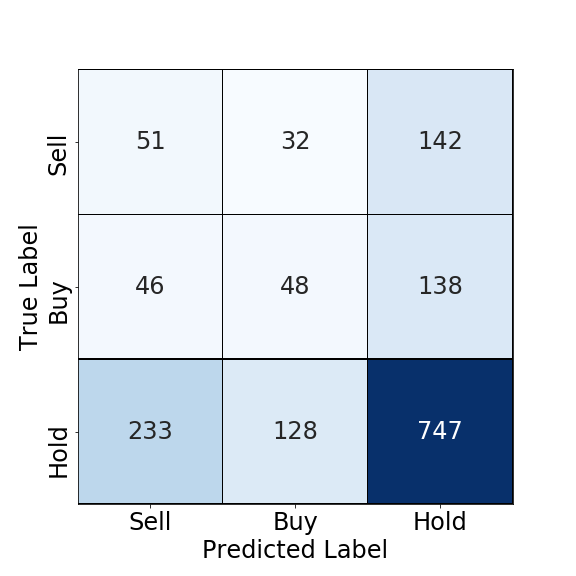
\includegraphics[width=.75\linewidth]{images/CMs/CM_indiv_GSPC.png}  
  \caption{S\&P500 asset-specific model}
  \label{fig:subGSPCI}
\end{subfigure}
\begin{subfigure}{.5\textwidth}
  \centering
  % include second image
  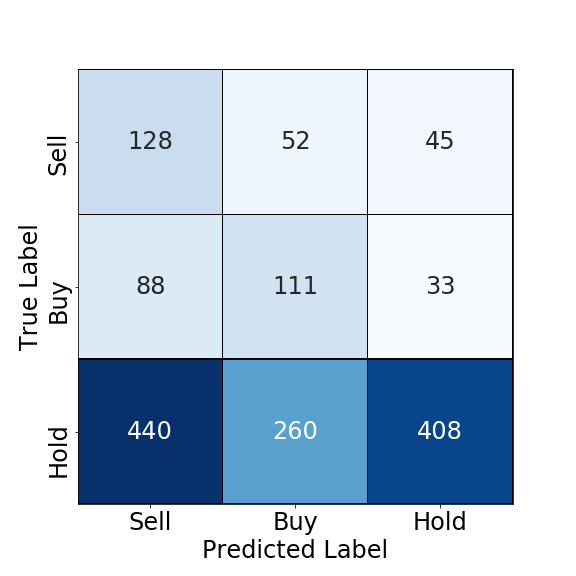
\includegraphics[width=.75\linewidth]{images/CMs/CM_univ_GSPC.png}  
  \caption{S\&P500 universal model}
  \label{fig:subGSPCU}
\end{subfigure}

\begin{subfigure}{.5\textwidth}
  \centering
  % include first image
  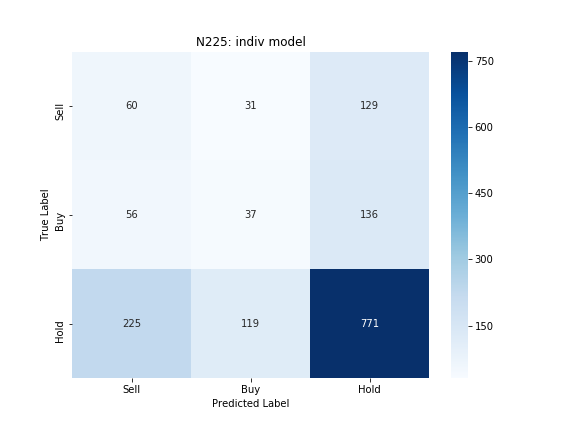
\includegraphics[width=.75\linewidth]{images/CMs/CM_indiv_N225.png}  
  \caption{Nikkei 225 asset-specific model}
  \label{fig:subN225I}
\end{subfigure}
\begin{subfigure}{.5\textwidth}
  \centering
  % include second image
  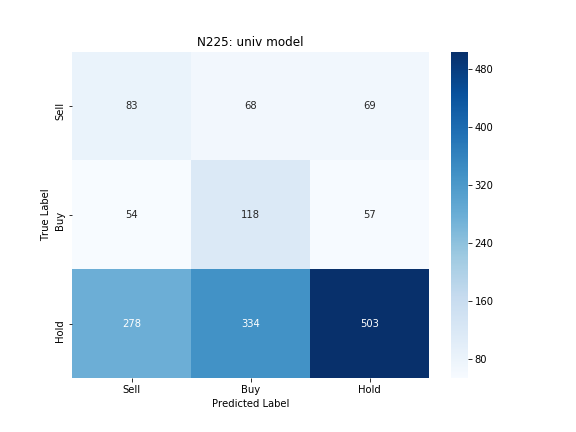
\includegraphics[width=.75\linewidth]{images/CMs/CM_univ_N225.png}  
  \caption{Nikkei 225 universal model}
  \label{fig:subN225U}
\end{subfigure}

\caption{Confusion matrices for S\&P500 and Nikkei 225 for each model variant, aggregated over testing periods}
\label{fig:AppCMs1}
\end{figure}

\begin{figure}[H]
\begin{subfigure}{.5\textwidth}
  \centering
  % include first image
  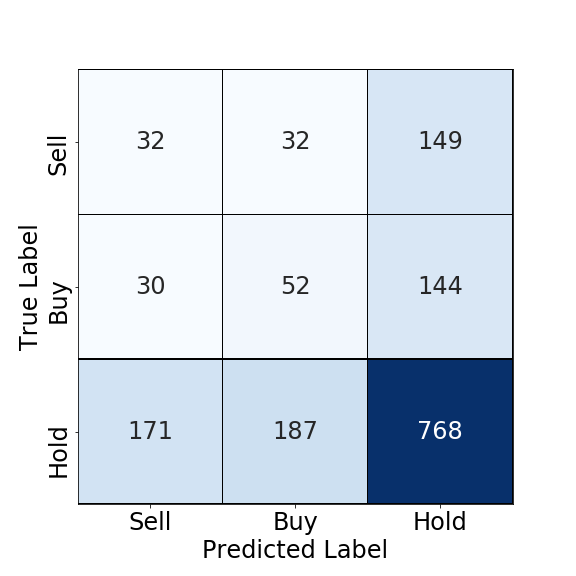
\includegraphics[width=.75\linewidth]{images/CMs/CM_indiv_IXIC.png}  
  \caption{Nasdaq asset-specific model}
  \label{fig:subIXICI}
\end{subfigure}
\begin{subfigure}{.5\textwidth}
  \centering
  % include second image
  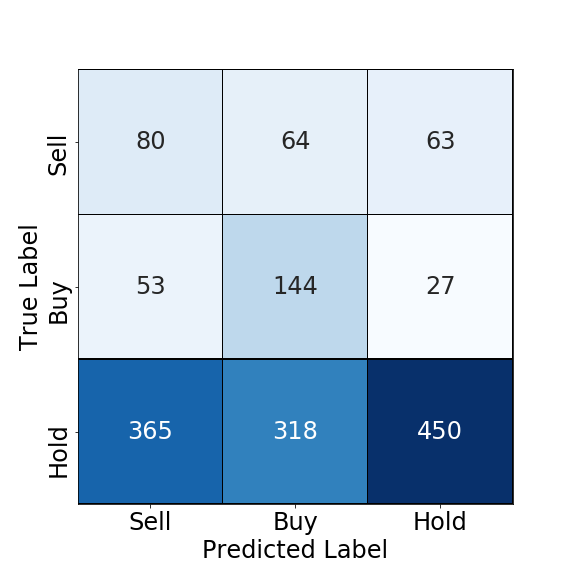
\includegraphics[width=.75\linewidth]{images/CMs/CM_univ_IXIC.png}  
  \caption{Nasdaq universal model}
  \label{fig:subIXICU}
\end{subfigure}

\begin{subfigure}{.5\textwidth}
  \centering
  % include first image
  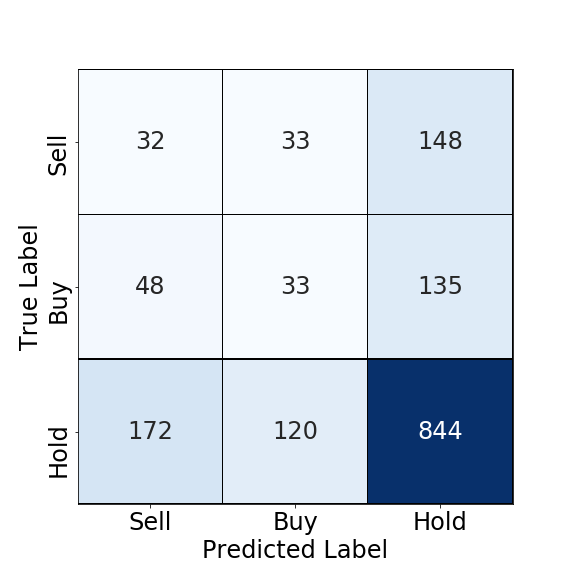
\includegraphics[width=.75\linewidth]{images/CMs/CM_indiv_AAPL.png}  
  \caption{Apple asset-specific model}
  \label{fig:subAAPLI}
\end{subfigure}
\begin{subfigure}{.5\textwidth}
  \centering
  % include second image
  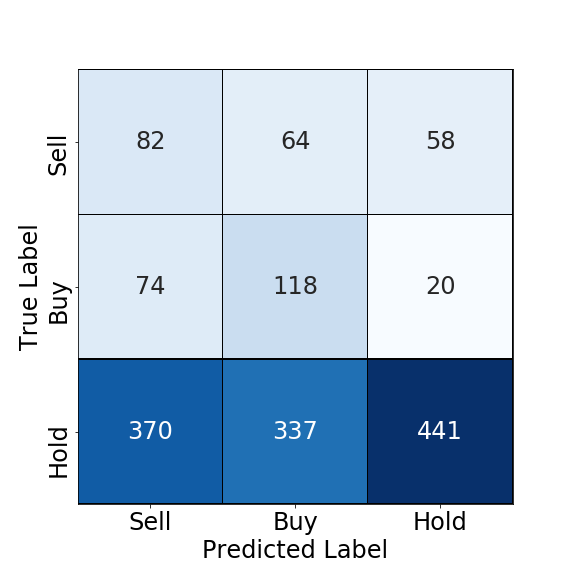
\includegraphics[width=.75\linewidth]{images/CMs/CM_univ_AAPL.png}  
  \caption{Apple universal model}
  \label{fig:subAAPLU}
\end{subfigure}

\begin{subfigure}{.5\textwidth}
  \centering
  % include first image
  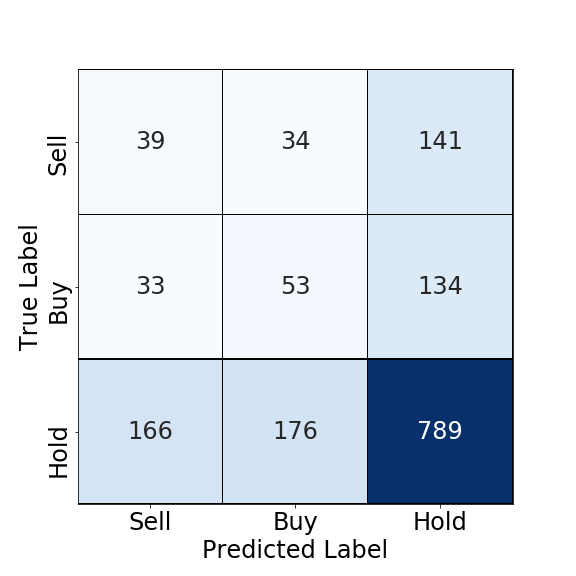
\includegraphics[width=.75\linewidth]{images/CMs/CM_indiv_SPY.png}  
  \caption{SPY ETF asset-specific model}
  \label{fig:subSPYI}
\end{subfigure}
\begin{subfigure}{.5\textwidth}
  \centering
  % include second image
  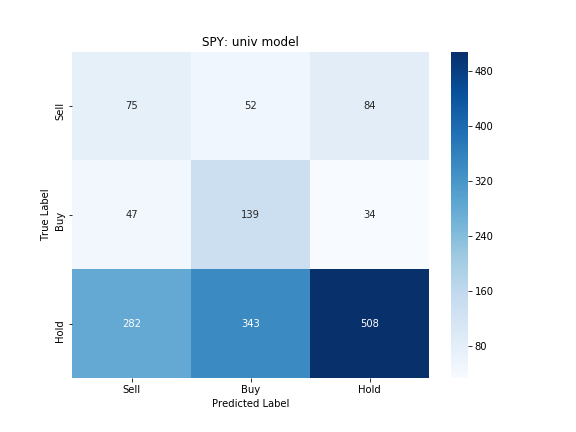
\includegraphics[width=.75\linewidth]{images/CMs/CM_univ_SPY.png}  
  \caption{SPY ETF universal model}
  \label{fig:subSPYU}
\end{subfigure}

\caption{Confusion matrices for Nasdaq, Apple and SPY ETF for each  model variant, aggregated over testing periods}
\label{fig:AppCMs2}
\end{figure}

\subsection{Data Sources}

The list of sources for all downloaded datasets can be found in Tables \ref{tbl:datasets_main}- \ref{tbl:datasets_commods}.

\begin{table}[H]
    \centering
        \begin{tabular}{p{3.0cm} p{10.0cm}l}
        \hline
        \textbf{Symbol}                                                             & \textbf{Source}                                                                                                                                              & \textbf{Date of Download} \\ \hline
       GSPC                                                                        & \url{https://finance.yahoo.com/quote/\%5EGSPC/history?period1=-630982800\&period2=1559944800\&interval=1d\&filter=history\&frequency=1d}    & June 8, 2019              \\
        N225                                                                        & \url{https://finance.yahoo.com/quote/\%5EN225/history?period1=-157424400\&period2=1559944800\&interval=1d\&filter=history\&frequency=1d}    & June 8, 2019              \\
        IXIC                                                                        & \url{https://finance.yahoo.com/quote/\%5EIXIC/history?period1=34556400\&period2=1559944800\&interval=1d\&filter=history\&frequency=1d}      & June 8, 2019              \\
        AAPL                                                                        & \url{https://finance.yahoo.com/quote/AAPL/history?period1=345423600\&period2=1559944800\&interval=1d\&filter=history\&frequency=1d}         & June 8, 2019              \\
        SPY                                                                         & \url{https://finance.yahoo.com/quote/SPY/history?period1=728262000\&period2=1559944800\&interval=1d\&filter=history\&frequency=1d}          & June 8, 2019              \\ \hline
        \end{tabular}
        \caption{Data sources: Testing datasets}
    \label{tbl:datasets_main}
\end{table}

        \begin{table}[H]
    \centering
        \begin{tabular}{p{3.0cm} p{10.0cm}l}
        \hline
        \textbf{Symbol}                                                             & \textbf{Source}                                                                                                                                              & \textbf{Date of Download} \\ \hline
       
        DJI                                                                         & \url{https://finance.yahoo.com/quote/\%5EDJI/history?period1=-630982800\&period2=1559944800\&interval=1d\&filter=history\&frequency=1d}     & June 8, 2019              \\
        GDAXI                                                                       & \url{https://finance.yahoo.com/quote/\%5EGDAXI/history?period1=567817200\&period2=1559944800\&interval=1d\&filter=history\&frequency=1d}    & June 8, 2019              \\
        SSI                                                                         & \url{https://finance.yahoo.com/quote/000001.SS/history?period1=661561200\&period2=1559944800\&interval=1d\&filter=history\&frequency=1d}    & June 8, 2019              \\
        VIX                                                                         & \url{https://finance.yahoo.com/quote/\%5EVIX/history?period1=631234800\&period2=1559944800\&interval=1d\&filter=history\&frequency=1d}      & June 8, 2019              \\
        INDEXFTSE: UKX                                                              & \url{https://www.londonstockexchange.com/statistics/ftse/ftse.htm}                                                                          & June 8, 2019              \\
        INDEXFTSE: MCX                                                              & \url{https://www.londonstockexchange.com/statistics/ftse/ftse.htm}                                                                          & June 8, 2019              \\
        INDEXFTSE: NMX                                                              & \url{https://www.londonstockexchange.com/statistics/ftse/ftse.htm}                                                                          & June 8, 2019              \\
        STOXX50E                                                                    & \url{https://finance.yahoo.com/quote/\%5ESTOXX50E/history?period1=536367600\&period2=1559944800\&interval=1d\&filter=history\&frequency=1d} & June 8, 2019              \\
        RUT                                                                         & \url{https://finance.yahoo.com/quote/\%5ERUT/history?period1=558223200\&period2=1559944800\&interval=1d\&filter=history\&frequency=1d}      & June 8, 2019              \\ \hline
        \end{tabular}
        \caption{Data sources: Stocks \& Indices}
        \label{tbl:datasets_stocks}
    \end{table}
    
        \begin{table}[H]
    \centering
        \begin{tabular}{p{3.0cm} p{10.0cm}l}
        \hline
        \textbf{Symbol}                                                             & \textbf{Source}                                                                                                                                              & \textbf{Date of Download} \\ \hline
        QQQ                                                                         & \url{https://finance.yahoo.com/quote/QQQ/history?period1=921020400\&period2=1559944800\&interval=1d\&filter=history\&frequency=1d}          & June 8, 2019              \\
        XLF                                                                         & \url{https://finance.yahoo.com/quote/XLF/history?period1=914281200\&period2=1559944800\&interval=1d\&filter=history\&frequency=1d}          & June 8, 2019              \\
        XLU                                                                         & \url{https://finance.yahoo.com/quote/XLU/history?period1=914281200\&period2=1559944800\&interval=1d\&filter=history\&frequency=1d}          & June 8, 2019              \\
        XLP                                                                         & \url{https://finance.yahoo.com/quote/XLP/history?period1=914281200\&period2=1559944800\&interval=1d\&filter=history\&frequency=1d}          & June 8, 2019              \\
        EWZ                                                                         & \url{https://finance.yahoo.com/quote/EWZ/history?period1=963525600\&period2=1559944800\&interval=1d\&filter=history\&frequency=1d}          & June 8, 2019              \\
        EWH                                                                         & \url{https://finance.yahoo.com/quote/EWH/history?period1=828309600\&period2=1559944800\&interval=1d\&filter=history\&frequency=1d}          & June 8, 2019              \\
        XLY                                                                         & \url{https://finance.yahoo.com/quote/XLY/history?period1=914281200\&period2=1559944800\&interval=1d\&filter=history\&frequency=1d}          & June 8, 2019              \\
        XLE                                                                         & \url{https://finance.yahoo.com/quote/XLE/history?period1=914281200\&period2=1559944800\&interval=1d\&filter=history\&frequency=1d}          & June 8, 2019              \\ \hline
        \end{tabular}
        \caption{Data sources: Exchange Traded Funds}
        \label{tbl:datasets_etfs}
    \end{table}
        
        \begin{table}[H]
    \centering
        \begin{tabular}{p{3.0cm} p{10.0cm}l}
        \hline
        \textbf{Symbol}                                                             & \textbf{Source}                                                                                                                                              & \textbf{Date of Download} \\ \hline
        DEXUSUK                                                                     & \url{https://fred.stlouisfed.org/categories/94}                                                                                             & June 8, 2019              \\
        DEXUSAL                                                                     & \url{https://fred.stlouisfed.org/categories/94}                                                                                             & June 8, 2019              \\
        DEXUSNZ                                                                     & \url{https://fred.stlouisfed.org/categories/94}                                                                                             & June 8, 2019              \\
        DEXUSEU                                                                     & \url{https://fred.stlouisfed.org/categories/94}                                                                                             & June 8, 2019              \\ \hline
       \end{tabular}
        \caption{Data sources: Foreign Exchange Rates}
        \label{tbl:datasets_FX}
    \end{table}
    
        \begin{table}[H]
    \centering
        \begin{tabular}{p{3.0cm} p{10.0cm}l}
        \hline
        \textbf{Symbol}                                                             & \textbf{Source}                                                                                                                                              & \textbf{Date of Download} \\ \hline
        
       Copper                                                                      & \url{https://www.macrotrends.net/1476/copper-prices-historical-chart-data}                                                                  & June 8, 2019              \\
        DCOILWTICO                                                                  & \url{https://fred.stlouisfed.org/graph/?g=NPX}                                                                                              & June 8, 2019              \\
        FOB                                                                         & \url{https://www.eia.gov/dnav/pet/hist\_xls/RBRTEd.xls}                                                                                     & June 8, 2019              \\
        XAUUSD                                                                      & \url{https://www.investing.com/currencies/xau-usd-historical-data}                                                                          & June 8, 2019              \\
        XAGUSD                                                                      & \url{https://www.investing.com/currencies/xag-usd-historical-data}                                                                          & June 8, 2019              \\
        Platinum                                                                    & \url{https://www.macrotrends.net/2540/platinum-prices-historical-chart-data}                                                                & June 8, 2019              \\
        Corn                                                                        & \url{https://www.macrotrends.net/2532/corn-prices-historical-chart-data}                                                                    & June 8, 2019              \\
        Coffee                                                                      & \url{https://www.macrotrends.net/2535/coffee-prices-historical-chart-data}                                                                  & June 8, 2019              \\
        Soybean oil                                                                 & \url{https://www.macrotrends.net/2538/soybean-oil-prices-historical-chart-data}                                                             & June 8, 2019              \\ \hline
        \end{tabular}
        \caption{Data sources: Commodities}
        \label{tbl:datasets_commods}
    \end{table}
   

\bibliography{reference}
\bibliographystyle{apalike}

\end{document}